\chapter{突触传递和神经元兴奋性的调节:第二信使} \label{chap:chap14}

神经递质与突触后受体的结合通过打开离子通道直接产生突触后电位,或通过改变突触后细胞生化状态改变离子通道活性间接产生突触后电位。
正如我们在第~\ref{chap:chap11}~章到第~\ref{chap:chap13}~章中看到的,突触后作用的类型取决于受体的类型。
\textit{离子型受体}的激活直接打开作为受体大分子本身一部分的离子通道。
相反,\textit{代谢型受体}的激活通过\textit{生化信号通路}间接调节离子通道的开放;
代谢型受体和受体调节的离子通道是不同的大分子(图~\ref{fig:14_1})。


% 翻译参考:https://zhuanlan.zhihu.com/p/95487714
\begin{figure}[htbp]
	\centering
	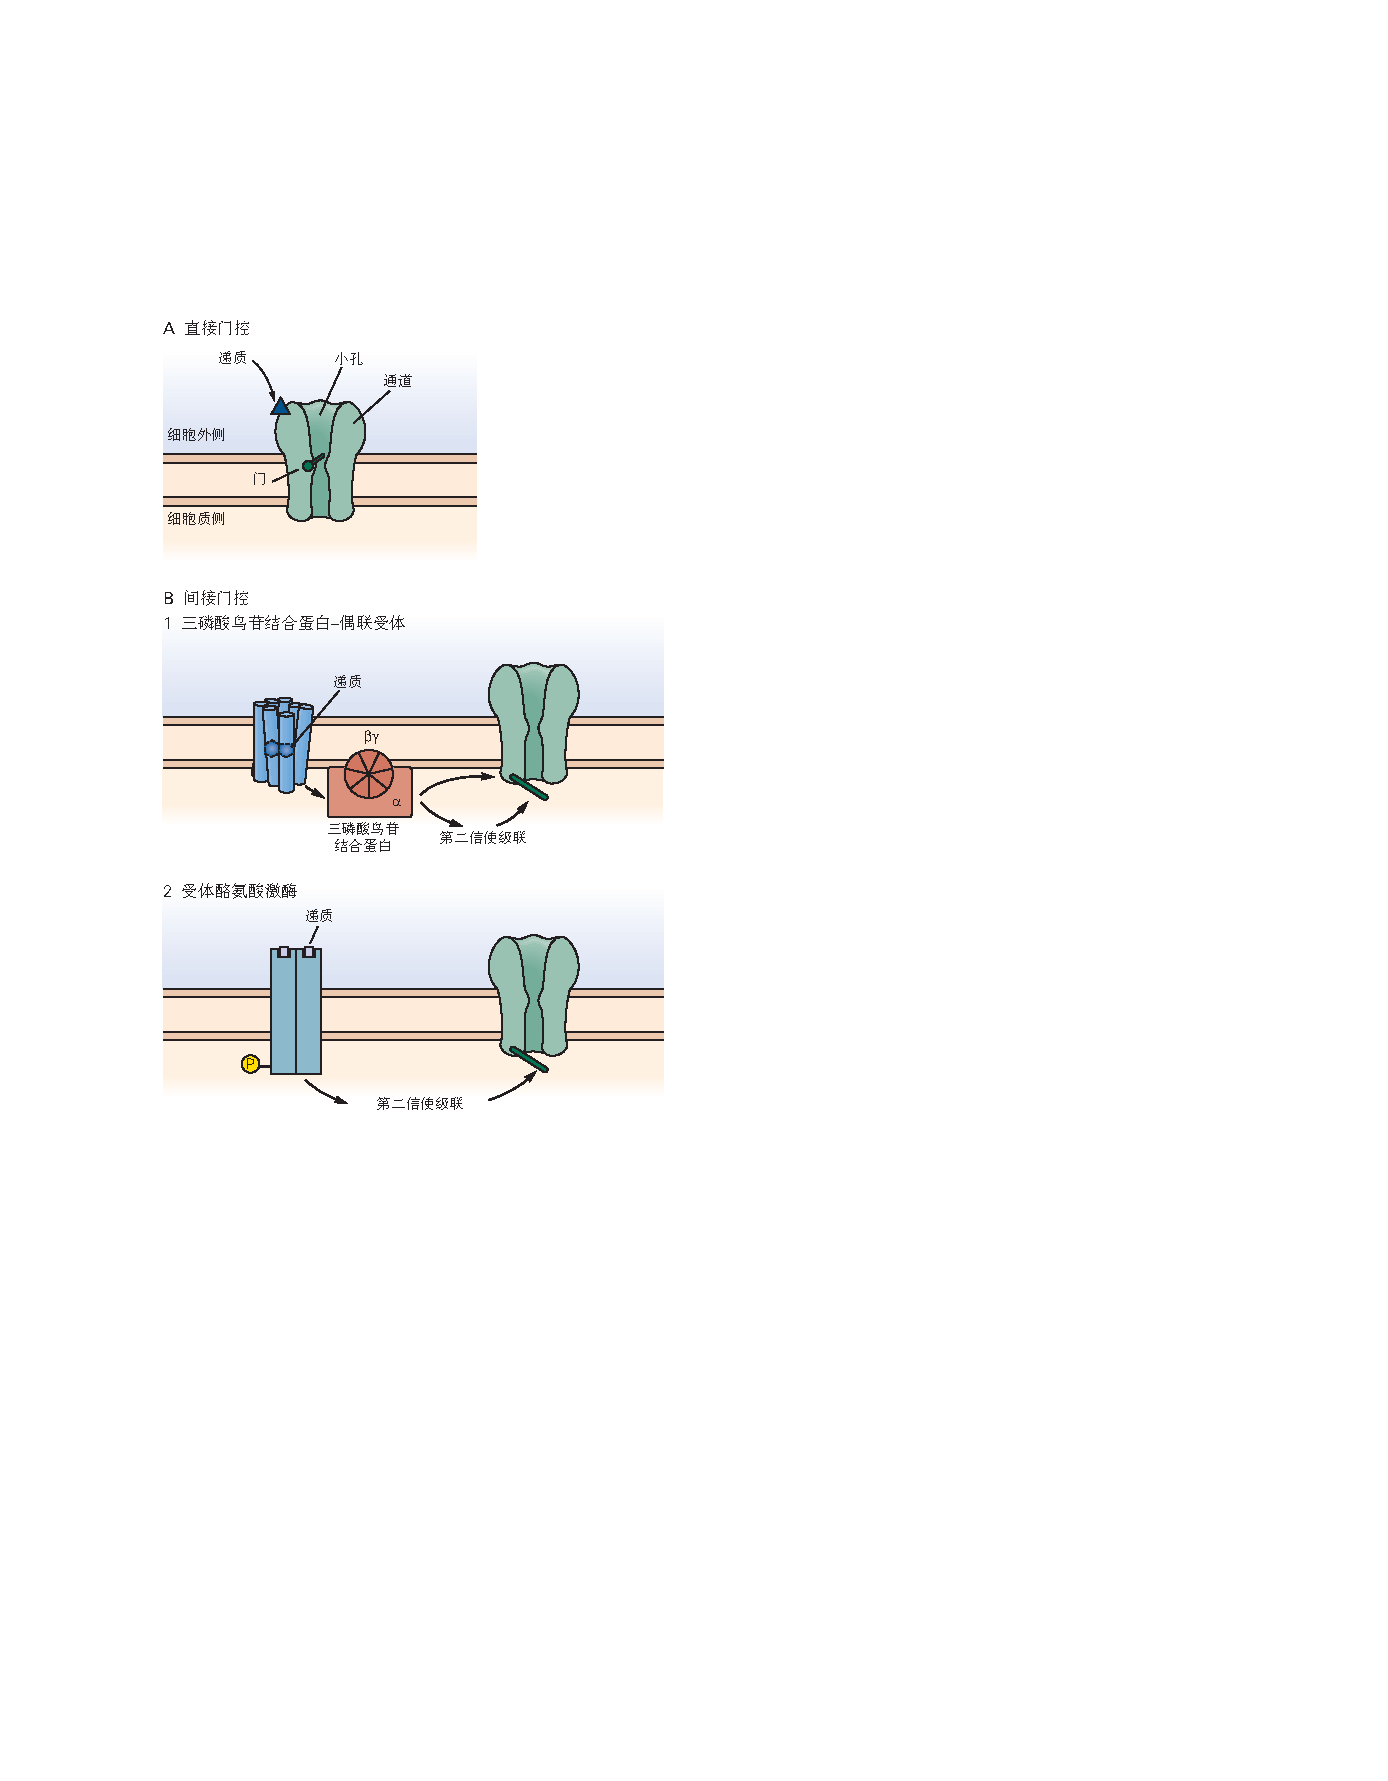
\includegraphics[width=0.5\linewidth]{chap14/fig_14_1}
	\caption{根据受体和效应器功能耦合的方式,神经递质作用可分为两组。
		\textbf{A.} 直接递质作用是通过\textit{递质}与离子型受体、配体门控\textit{通道}的结合产生的,其中受体和离子通道是单个大分子内的结构域。
		递质与受体通道蛋白细胞外受体的结合直接打开嵌入细胞膜的离子通道。
		\textbf{B.} 间接递质作用是由\textit{递质}与代谢受体结合引起的,代谢受体是与它们调节的离子通道分开的大分子。
		这些受体有两个家族。
		\textbf{1.} 三磷酸鸟苷结合蛋白–偶联受体激活\textit{三磷酸鸟苷结合蛋白},这些蛋白参与第二信使级联或直接作用于离子通道。
		\textbf{2.} 受体酪氨酸激酶启动一系列蛋白质磷酸化反应,首先是激酶本身在酪氨酸残基上的自磷酸化。}
	\label{fig:14_1}
\end{figure}


离子型受体的作用\textit{快速}而\textit{短暂},而代谢型受体产生的作用开始\textit{缓慢}并持续很长时间,从数百毫秒到数分钟不等。
这两种受体的功能也不同。
离子型受体是快速突触信号的基础,它是所有行为的基础,从简单的反射到复杂的认知过程。
代谢受体调节行为;
它们改变反射强度,激活运动模式,集中注意力,设定情绪状态,并有助于构成学习和记忆基础的神经回路的长期变化。
\textit{代谢型受体}负责递质、激素和生长因子的许多作用。
这些神经调节剂的作用可以在神经元兴奋性和突触强度方面产生显着和显着的变化,并且这样做可以深刻地改变对行为很重要的整个回路中的活动状态。


离子型受体迅速改变膜电位。
正如我们所见,这种变化起初是局部的,但如果膜电位的变化是超阈值的,则这种变化会作为动作电位沿轴突传播。
代谢受体的激活也开始于局部作用,可以扩散到细胞的更广泛区域。
神经递质与\textit{代谢型受体}的结合会激活蛋白质,进而激活\textit{效应酶}。
然后,效应酶通常会产生\textit{第二信使}分子,这些分子可以在\textit{细胞内}扩散以激活其他酶,这些酶可以催化各种靶蛋白的修饰,从而极大地改变它们的活性。


有两个主要的\textit{代谢型受体}家族:G 蛋白偶联受体和受体酪氨酸激酶。
我们首先描述 G 蛋白偶联受体家族,然后讨论受体酪氨酸激酶家族。


G 蛋白偶联受体通过三聚体鸟嘌呤核苷酸结合蛋白或 G 蛋白与效应子偶联(图~\ref{fig:14_1}B)。
该受体家族包括去甲肾上腺素的$\alpha$- 和 $\beta$-肾上腺素能受体、毒蕈碱型\textit{乙酰胆碱}受体、\textit{$\gamma$-氨基丁酸 B}受体、某些谷氨酸和血清素受体、多巴胺的所有受体、神经肽受体、气味受体、视紫红质 (对光起反应的蛋白质,启动视觉信号);
见第~\ref{chap:chap22}~章)和许多其他。
许多这些受体被认为与神经和精神疾病有关,并且是重要治疗药物类别作用的关键靶标。


G 蛋白偶联受体可激活多种效应器。
典型的效应器是产生可扩散第二信使的酶。
这些第二信使反过来触发生化级联反应,通过激活磷酸化各种蛋白质中特定丝氨酸或苏氨酸残基的羟基的特定蛋白激酶,或通过动员细胞内储存的~\ce{Ca^2+} 离子,从而启动改变细胞生化状态的反应。
在某些情况下,G 蛋白或第二信使直接作用于离子通道。



\section{\textit{环磷酸腺苷}通路是了解最多的由 G 蛋白偶联受体启动的第二信使信号级联}

腺苷 3',5'-环磷酸(\textit{环磷酸腺苷}或\textit{环磷酸腺苷})途径是 G 蛋白偶联的第二信使级联的原型示例。
它是第一个被发现的第二信使通路,我们对其他第二信使通路的概念也是基于它。


递质与连接到\textit{环磷酸腺苷}级联的受体的结合首先激活特定的 G 蛋白 $ G_s $(因其刺激\textit{环磷酸腺苷}合成的作用而得名)。
在静息状态下,$ G_s $ 与所有 G 蛋白一样,是由$\alpha$-、$\beta$- 和 $\gamma$- 亚基组成的三聚体蛋白。
$\alpha$-亚基仅与膜松散结合,通常是将受体与其主要效应酶偶联的试剂。
$\beta$- 和 $\gamma$- 亚基形成与膜更紧密结合的强结合复合物。
正如本章后面所述,G 蛋白的 $\beta \gamma$ 复合体可以直接调节某些离子通道的活性。


在静息状态下,$\alpha$-亚基结合\textit{二磷酸鸟苷}分子。
在配体结合后,G 蛋白偶联受体发生构象变化,使其能够与$\alpha$亚基结合,从而促进\textit{二磷酸鸟苷}与\textit{三磷酸鸟苷}分子的交换。
这导致构象变化,导致$\alpha$-亚基与 $\beta \gamma$ 复合物分离,从而激活 $\alpha$-亚基。


与\textit{环磷酸腺苷}级联偶联的特定类别的$\alpha$-亚基称为$\alpha_s$,它刺激整合膜蛋白腺苷酸环化酶催化\textit{三磷酸腺苷}转化为\textit{环磷酸腺苷}。
当与环化酶结合时,$\alpha_s$ 也充当\textit{三磷酸鸟苷}酶,将其结合的\textit{三磷酸鸟苷}水解为\textit{二磷酸鸟苷}。
当\textit{三磷酸鸟苷}水解时,$\alpha_s$ 失去活性。
它从腺苷酸环化酶解离并与 $\beta \gamma$ 复合物重新结合,从而停止\textit{环磷酸腺苷}的合成(图~\ref{fig:14_2}A)。
$ G_s $ 蛋白通常在其结合的\textit{三磷酸鸟苷}水解之前保持活性几秒钟。


\begin{figure}[htbp]
	\centering
	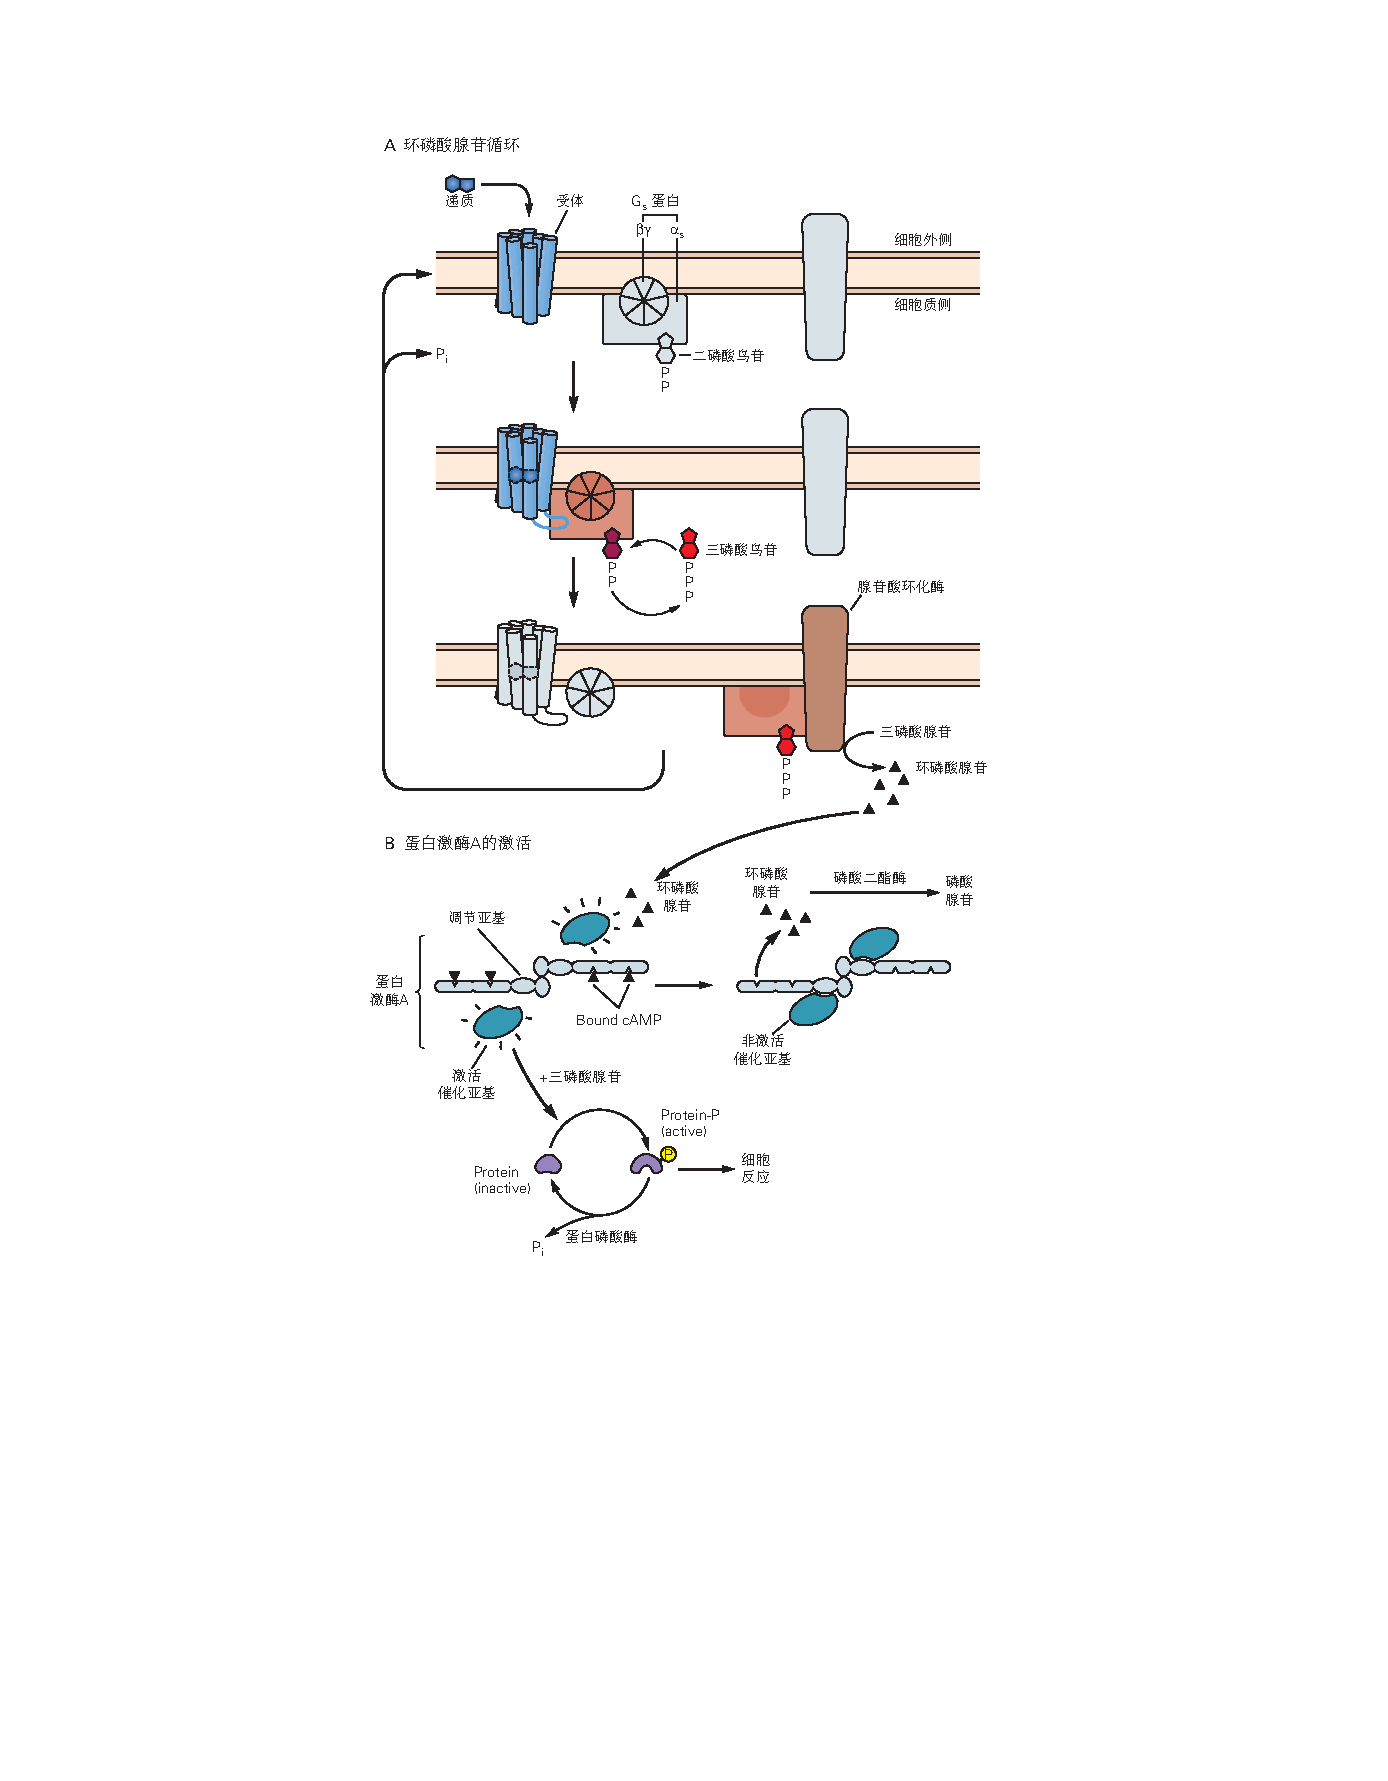
\includegraphics[width=0.65\linewidth]{chap14/fig_14_2}
	\caption{G 蛋白偶联受体的激活会刺激\textit{环磷酸腺苷}的产生和蛋白激酶 A\cite{alberts2017molecular}。
		\textbf{A.} 递质与某些受体的结合会激活刺激性 G 蛋白 ($ G_s $),包括 $\alpha_s$-、$\beta$-和 $\gamma$-亚基。
		当被激活时,$\alpha_s$ 亚基将其结合的\textit{二磷酸鸟苷}交换为\textit{三磷酸鸟苷},导致$\alpha_s$ 从 $\beta \gamma$ 复合物中解离。
		接下来,$\alpha_s$ 与腺苷酸环化酶的胞内结构域结合,从而刺激该酶从\textit{三磷酸腺苷}产生\textit{环磷酸腺苷}。
		\textit{三磷酸鸟苷}水解为\textit{二磷酸鸟苷}和无机磷酸盐 ($ P_i $) 导致$\alpha_s$ 从环化酶解离并与 $\beta \gamma$ 复合物重新结合。
		然后环化酶停止产生第二信使。
		当递质与受体分离时,G 蛋白的三个亚基重新结合,$\alpha$亚基上的鸟嘌呤核苷酸结合位点被\textit{二磷酸鸟苷}占据。
		\textbf{B.} 四个\textit{环磷酸腺苷}分子与\textit{蛋白激酶A}的两个调节亚基结合,释放两个催化亚基,然后自由磷酸化某些丝氨酸或苏氨酸残基上的特定底物蛋白,从而调节蛋白质功能以产生给定的细胞回复。
		有两种酶调节该途径。
		磷酸二酯酶将\textit{环磷酸腺苷}转化为腺苷一磷酸(无活性),蛋白磷酸酶从底物蛋白中去除磷酸基团 (P),释放无机磷酸盐 $ P_i $。
		当磷酸酶被\textit{蛋白激酶A}磷酸化时,其活性又会被蛋白抑制剂 1(未显示)降低。}
	\label{fig:14_2}
\end{figure}


一旦 G 蛋白偶联受体与配体结合,它就可以依次与多个 G 蛋白大分子相互作用。
结果,相对较少的递质分子与少量受体的结合可以激活大量环化酶复合物。
该信号在\textit{环磷酸腺苷}级联的下一步中进一步放大,即蛋白激酶的激活。


大多数细胞中\textit{环磷酸腺苷}的主要靶标是\textit{环磷酸腺苷}依赖性蛋白激酶(也称为\textit{蛋白激酶A})。
这种由 Edward Krebs 及其同事鉴定和表征的激酶是一种异四聚体酶,由两个调节 (R) 亚基和两个催化 (C) 亚基的二聚体组成。
在没有\textit{环磷酸腺苷}的情况下,R 亚基结合并抑制 C 亚基。
在\textit{环磷酸腺苷}存在的情况下,每个 R 亚基结合两个\textit{环磷酸腺苷}分子,导致构象变化,导致 R 和 C 亚基解离(图~\ref{fig:14_2}B)。
解离释放 C 亚基,将\textit{三磷酸腺苷}的 $\gamma$-磷酰基转移到底物蛋白中特定丝氨酸和苏氨酸残基的羟基。
\textit{蛋白激酶A}的作用被磷蛋白磷酸酶终止,磷蛋白磷酸酶是从蛋白质中裂解磷酸基团,产生无机磷酸盐的酶。


蛋白激酶 A 通过进化与我们将考虑的其他丝氨酸和苏氨酸蛋白激酶有远亲关系:钙/钙调蛋白依赖性蛋白激酶和蛋白激酶 C。
这些激酶也有调节和催化结构域,但这两个结构域都在同一多肽中 分子(见图~\ref{fig:14_4})。


\begin{figure}[htbp]
	\centering
	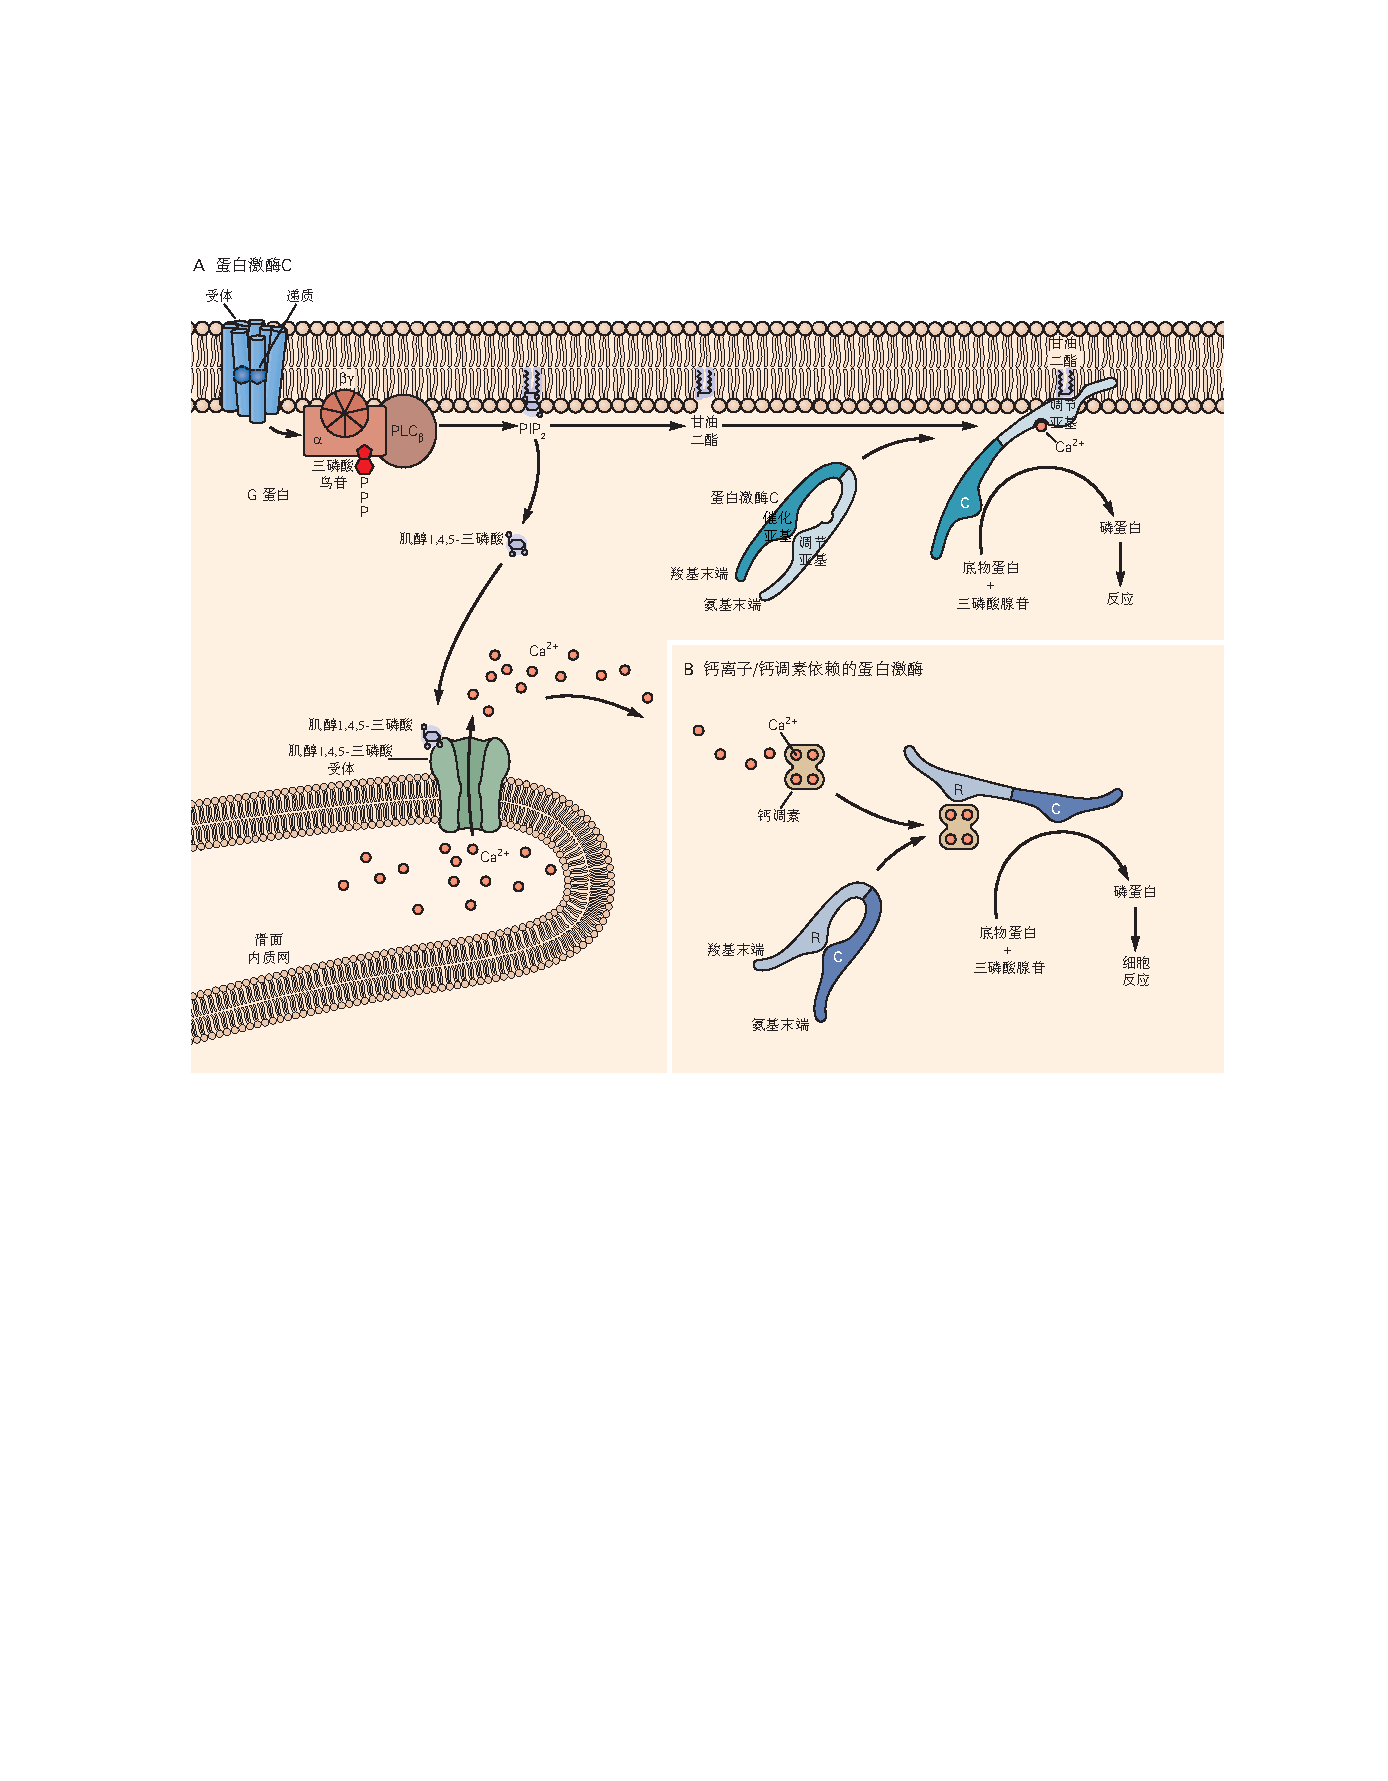
\includegraphics[width=0.95\linewidth]{chap14/fig_14_4}
	\caption{细胞膜中磷脂的水解激活三个主要的第二信使级联反应。
		\textbf{A.} 递质与受体的结合激活了激活磷脂酶 C$\beta$ (PLC$\beta$) 的 G 蛋白。
		这种酶将磷脂酰肌醇 4,5-二磷酸 (PIP2) 裂解成第二信使\textit{肌醇1,4,5-三磷酸}和二酰甘油 (DAG)。
		\textit{肌醇1,4,5-三磷酸}是水溶性的并扩散到细胞质中,在那里它与光滑内质网上的\textit{肌醇1,4,5-三磷酸}受体通道结合,从而从内部储存中释放 \ce{Ca^2+}。
		DAG 保留在膜中,在那里它募集并激活蛋白激酶 C (PKC)。
		膜磷脂也是 PKC 激活所必需的辅助因子。
		PKC 的一些亚型也需要 \ce{Ca^2+} 才能激活。
		PKC 由单个蛋白质分子组成,该分子具有结合 DAG 的调节结构域和使丝氨酸或苏氨酸残基上的蛋白质磷酸化的催化结构域。
		在没有 DAG 的情况下,调节域会抑制催化域。
		\textbf{B.} 当 \ce{Ca^2+} 与钙调蛋白结合时,钙/钙调蛋白依赖性蛋白激酶被激活,然后钙/钙调蛋白复合物与激酶的调节域结合。
		该激酶由许多相似的亚基组成(此处仅显示其中一个),每个亚基都具有调节和催化功能。
		催化结构域磷酸化丝氨酸或苏氨酸残基上的蛋白质。
		(ATP,三磷酸腺苷;C,催化亚基;COOH,羧基末端;H2N,氨基末端;R,调节亚基。)}
	\label{fig:14_4}
\end{figure}


除了阻断酶活性外,\textit{蛋白激酶A}的调节亚基还将催化亚基靶向细胞内的不同位点。
人类\textit{蛋白激酶A}有两种类型的 R 亚基,RI 和 RII,每一种都有两种亚型:RI$\alpha$、RI$\beta$、RII$\alpha$ 和 RII$\beta$。
每个人的基因都来自一个共同的祖先,但具有不同的特性。
例如,II 型\textit{蛋白激酶A}(包含 RII 型亚基)通过 A 激酶附着蛋白 (AKAP) 靶向膜。
一种类型的 AKAP 通过结合\textit{蛋白激酶A}和突触后密度蛋白 PSD-95,将\textit{蛋白激酶A}靶向\textit{N-甲基-D-天冬氨酸}型谷氨酸受体,PSD-95 结合 NMDA 受体的细胞质尾部(第~\ref{chap:chap13}~章)。
此外,该 AKAP 还结合蛋白磷酸酶,该酶从底物蛋白中去除磷酸基团。
通过将\textit{蛋白激酶A}和其他信号成分定位在其底物附近,AKAP 形成局部信号复合物,从而提高第二信使级联的特异性、速度和效率。
因为 AKAP 对 RI 亚基的亲和力很弱,所以大多数 I 型\textit{蛋白激酶A}在细胞质中是游离的。


激酶只能磷酸化嵌入在氨基酸特定磷酸化共有序列范围内的丝氨酸和苏氨酸残基上的蛋白质。
例如,\textit{蛋白激酶A}的磷酸化通常需要两个连续的碱性氨基酸(赖氨酸或精氨酸)的序列,后跟任何氨基酸,然后是被磷酸化的丝氨酸或苏氨酸残基(例如,Arg-Arg-Ala-Thr )。


已在神经元中鉴定出几种重要的\textit{蛋白激酶A}蛋白质底物。
这些包括电压门控和配体门控离子通道、突触小泡蛋白、参与递质生物合成的酶以及调节基因转录的蛋白质。
因此,\textit{环磷酸腺苷}通路对神经元的电生理和生化特性具有广泛的影响。
我们将在本章后面考虑其中的一些操作。



\section{由 G 蛋白偶联受体启动的第二信使通路具有共同的分子逻辑}

人类基因组中大约 3.5\% 的基因编码 G 蛋白偶联受体。
尽管其中许多是嗅觉神经元中的气味受体(第 ~\ref{chap:chap29}~章),但许多其他受体是用于整个神经系统的特征明确的神经递质的受体。
尽管它们具有巨大的多样性,但所有 G 蛋白偶联受体都由具有七个特征性跨膜区域(蛇形受体)的单一多肽组成(图~\ref{fig:14_3}A)。
X 射线晶体学的最新结果提供了对这些与其各自 G 蛋白接触的受体的三维结构的详细见解(图~\ref{fig:14_3} B)。


\begin{figure}[htbp]
	\centering
	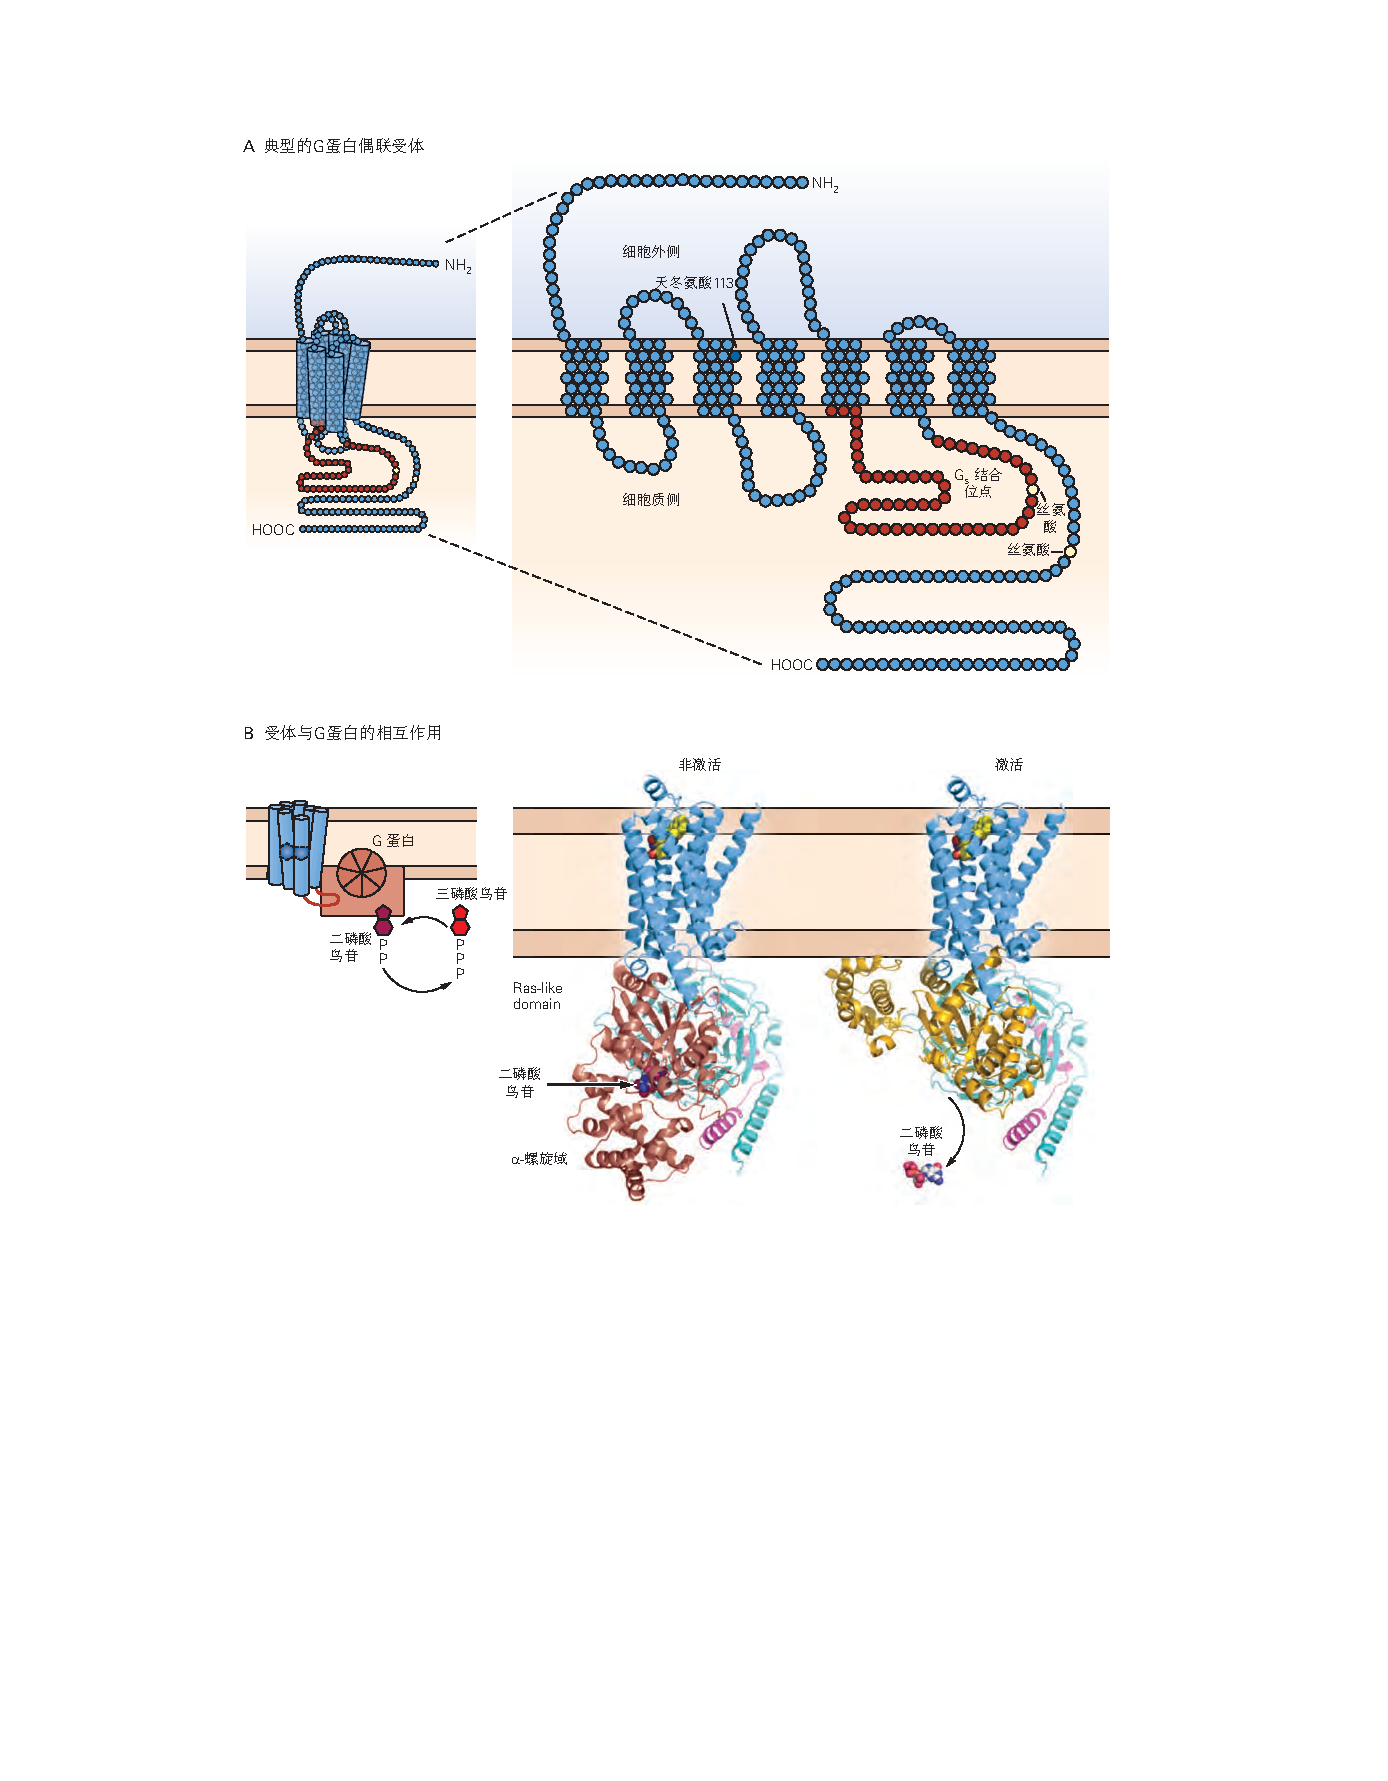
\includegraphics[width=0.75\linewidth]{chap14/fig_14_3}
	\caption{G 蛋白偶联受体包含七个跨膜结构域。
		\textbf{A.} 此处显示的 $\beta$2-肾上腺素能受体代表 G 蛋白偶联受体,包括 $\beta$1-肾上腺素能和毒蕈碱型\textit{乙酰胆碱}受体以及视紫红质。
		它由一个具有细胞外氨基末端、细胞内羧基末端和七个跨膜 $\alpha$螺旋的亚基组成。
		神经递质的结合位点位于受体中由跨膜螺旋形成的裂缝中。
		氨基酸残基天冬氨酸 (Asp)-113 参与结合。
		以棕色表示的受体部分与 $ G_s $ 蛋白$\alpha$亚基相关。
		细胞内羧基末端尾部的两个丝氨酸 (Ser) 残基是特定受体激酶磷酸化的位点,有助于使受体失活\cite{frielle1989beta}。
		\textbf{B.} 基于 $\beta$2-肾上腺素能受体(蓝色)与处于非活性\textit{二磷酸鸟苷}结合状态的 $ G_s $ 蛋白相互作用的 X 射线晶体结构的模型和 活性\textit{三磷酸鸟苷}结合状态。
		高亲和力合成激动剂结合在膜细胞外表面附近的跨膜区域(空间填充模型)。
		无活性 $ G_s $ 蛋白的$\alpha_s$-、$\beta$- 和 $\gamma$- 亚基分别以棕色、青色和紫色显示。
		在活性状态下,$\alpha_s$(金)会发生构象变化,使其能够与腺苷酸环化酶相互作用\cite{kobilka2013structural}。}
	\label{fig:14_3}
\end{figure}


在突触传递中充当第二信使的物质数量远少于递质数量。 超过100种物质作为递质;
每一种都可以激活存在于不同细胞中的几种类型的受体。
已被充分表征的少数第二信使分为两类,细胞内和跨细胞。
细胞内信使是一种分子,其作用仅限于产生它们的细胞。 
跨细胞信使是可以轻易穿过细胞膜的分子,因此可以离开产生它们的细胞,作为细胞间信号或相邻细胞的第一信使。


\subsection{G 蛋白家族激活不同的第二信使通路}

已鉴定出约 20 种$\alpha$-亚基、5 种 $\beta$-亚基和 12 种 $\gamma$-亚基。
具有不同 $\alpha$ 亚基的 G 蛋白偶联不同类别的受体和效应器,因此具有不同的生理作用。
例如,含有 $\alpha$i 亚基的抑制性 Gi 蛋白可抑制腺苷酸环化酶并降低\textit{环磷酸腺苷}水平。
其他 G 蛋白(Gq/11 蛋白,包含 $\alpha$q- 或 $\alpha$11- 亚基)激活磷脂酶 C,可能还有其他尚未确定的信号转导机制。
含有 $\alpha$o 亚基的 Go 蛋白在大脑中的表达水平特别高,但其确切目标尚不清楚。
与身体的其他器官相比,大脑含有异常丰富的 G 蛋白。
即便如此,由于与数量更多的受体相比,G 蛋白的类别数量有限,因此一种类型的 G 蛋白通常可以被不同类别的受体激活。


G 蛋白的已知效应靶标的数量甚至比 G 蛋白的类型还要有限。
重要的效应器包括某些被 $\beta \gamma$ 复合物激活的离子通道、\textit{环磷酸腺苷}通路中的腺苷酸环化酶、二酰基甘油-肌醇多磷酸通路中的磷脂酶 C 和花生四烯酸通路中的磷脂酶 A2。
这些效应器中的每一个(离子通道除外)都会引发细胞内特定靶蛋白的变化,或者通过产生与靶蛋白结合的第二信使,或者通过激活使其磷酸化的蛋白激酶。



\subsection{磷脂酶 C 水解磷脂产生两个重要的第二信使,\textit{肌醇1,4,5-三磷酸}和甘油二酯}

许多重要的第二信使是通过质膜内层磷脂的水解产生的。 
这种水解由三种酶——磷脂酶 C、D 和 A2——以它们在磷脂中水解的酯键命名。
每种磷脂酶都可以被与不同受体偶联的不同 G 蛋白激活。


最常见的水解磷脂是磷脂酰肌醇 4,5-二磷酸酯 (PIP2),它通常包含在第一个位置酯化到甘油主链上的脂肪酸硬脂酸酯和在第二个位置上酯化的不饱和脂肪酸花生四烯酸酯。
激活与 Gq 或 G11 偶联的受体会刺激磷脂酶 C,从而导致 PIP2 水解(特别是将甘油主链连接到极性头基的磷酸二酯键)并产生两个第二信使二酰基甘油 (DAG) 和\textit{肌醇1,4,5-三磷酸}。


疏水性甘油二酯在形成时保留在膜中,在那里它募集细胞质蛋白激酶 C (PKC)。
PKC 与 DAG 和某些膜磷脂一起形成一种活性复合物,可以磷酸化细胞中的许多蛋白质底物,包括膜相关蛋白和细胞质蛋白(图~\ref{fig:14_4} A)。
除 DAG 外,某些 PKC 同种型的激活还需要细胞质 \ce{Ca^2+} 水平升高。


磷脂酶 C 途径的第二个产物\textit{肌醇1,4,5-三磷酸}刺激平滑内质网腔中细胞内膜储存的 \ce{Ca^2+} 释放。
网状细胞膜包含一个大的完整膜大分子,即\textit{肌醇1,4,5-三磷酸}受体,它在其细胞质表面形成\textit{肌醇1,4,5-三磷酸}受体和跨越网状细胞膜的 \ce{Ca^2+} 通道。
当这个大分子结合\textit{肌醇1,4,5-三磷酸}时,通道打开,将 \ce{Ca^2+} 释放到细胞质中(图~\ref{fig:14_4}A)。


细胞内 \ce{Ca^2+} 的增加会触发许多生化反应并打开质膜中的钙门控通道。
钙还可以作为第二信使,通过与光滑内质网膜中的另一种整合蛋白兰尼碱受体(之所以这样称呼是因为它与植物生物碱兰尼碱结合,从而抑制 受体;
相反,咖啡因会打开兰尼碱受体)。
与它的远亲\textit{肌醇1,4,5-三磷酸}受体一样,兰尼碱受体形成一个跨越网状膜的 \ce{Ca^2+} 通道;
然而,细胞质 \ce{Ca^2+} 而不是\textit{肌醇1,4,5-三磷酸}打开兰尼碱受体通道。


钙通常通过与细胞质小蛋白钙调蛋白结合起作用。
钙/钙调蛋白复合物的一个重要功能是激活钙/钙调蛋白依赖性蛋白激酶(CaM 激酶)。
这种酶是许多相似亚基的复合体,每个亚基在同一多肽链中都包含调节域和催化域。
当钙/钙调蛋白复合物不存在时,激酶的 C 端调节域结合并使催化部分失活。
与钙/钙调蛋白复合物的结合导致激酶分子的构象变化,从而解除对催化结构域的作用(图~\ref{fig:14_4} B)。
一旦被激活,CaM 激酶可以通过分子内许多位点的分子内反应磷酸化自身。
自磷酸化有一个重要的功能作用:它将酶转化为一种独立于钙/钙调蛋白的形式,因此即使在没有 \ce{Ca^2+} 的情况下也能持续保持活性。


蛋白激酶的持续激活是维持生化过程的一种普遍且重要的机制,生化过程是与某些形式的记忆相关的突触功能长期变化的基础。
除了钙/钙调蛋白依赖性蛋白激酶的持续激活外,由于游离调节亚基通过泛素途径的酶促降解缓慢,\textit{蛋白激酶A}也可以在\textit{环磷酸腺苷}长时间增加后持续活跃。
调节亚基浓度的下降导致游离催化亚基的长期存在,即使在\textit{环磷酸腺苷}水平下降之后,也会导致底物蛋白的持续磷酸化。
PKC 也可以通过其调节和催化结构域的蛋白水解切割或通过缺乏调节结构域的 PKC 亚型的表达而变得持续活跃。
最后,磷酸化的持续时间可以通过某些起到抑制磷蛋白磷酸酶活性作用的蛋白质来增强。
一种这样的蛋白质,抑制剂-1,仅当抑制剂本身被\textit{蛋白激酶A}磷酸化时才抑制磷酸酶活性。



\section{受体酪氨酸激酶构成代谢受体的第二大家族}

受体酪氨酸激酶代表了与 G 蛋白偶联受体不同的受体家族。
受体酪氨酸激酶是由单个亚基组成的完整膜蛋白,该亚基具有通过单个跨膜片段连接到细胞质区域的胞外配体结合结构域。
细胞质区域包含一个蛋白激酶结构域,该结构域磷酸化自身(自磷酸化)和酪氨酸残基上的其他蛋白质(图 ~\ref{fig:14_5} A)。
这种磷酸化导致大量蛋白质的激活,包括能够作用于离子通道的其他激酶。


\begin{figure}[htbp]
	\centering
	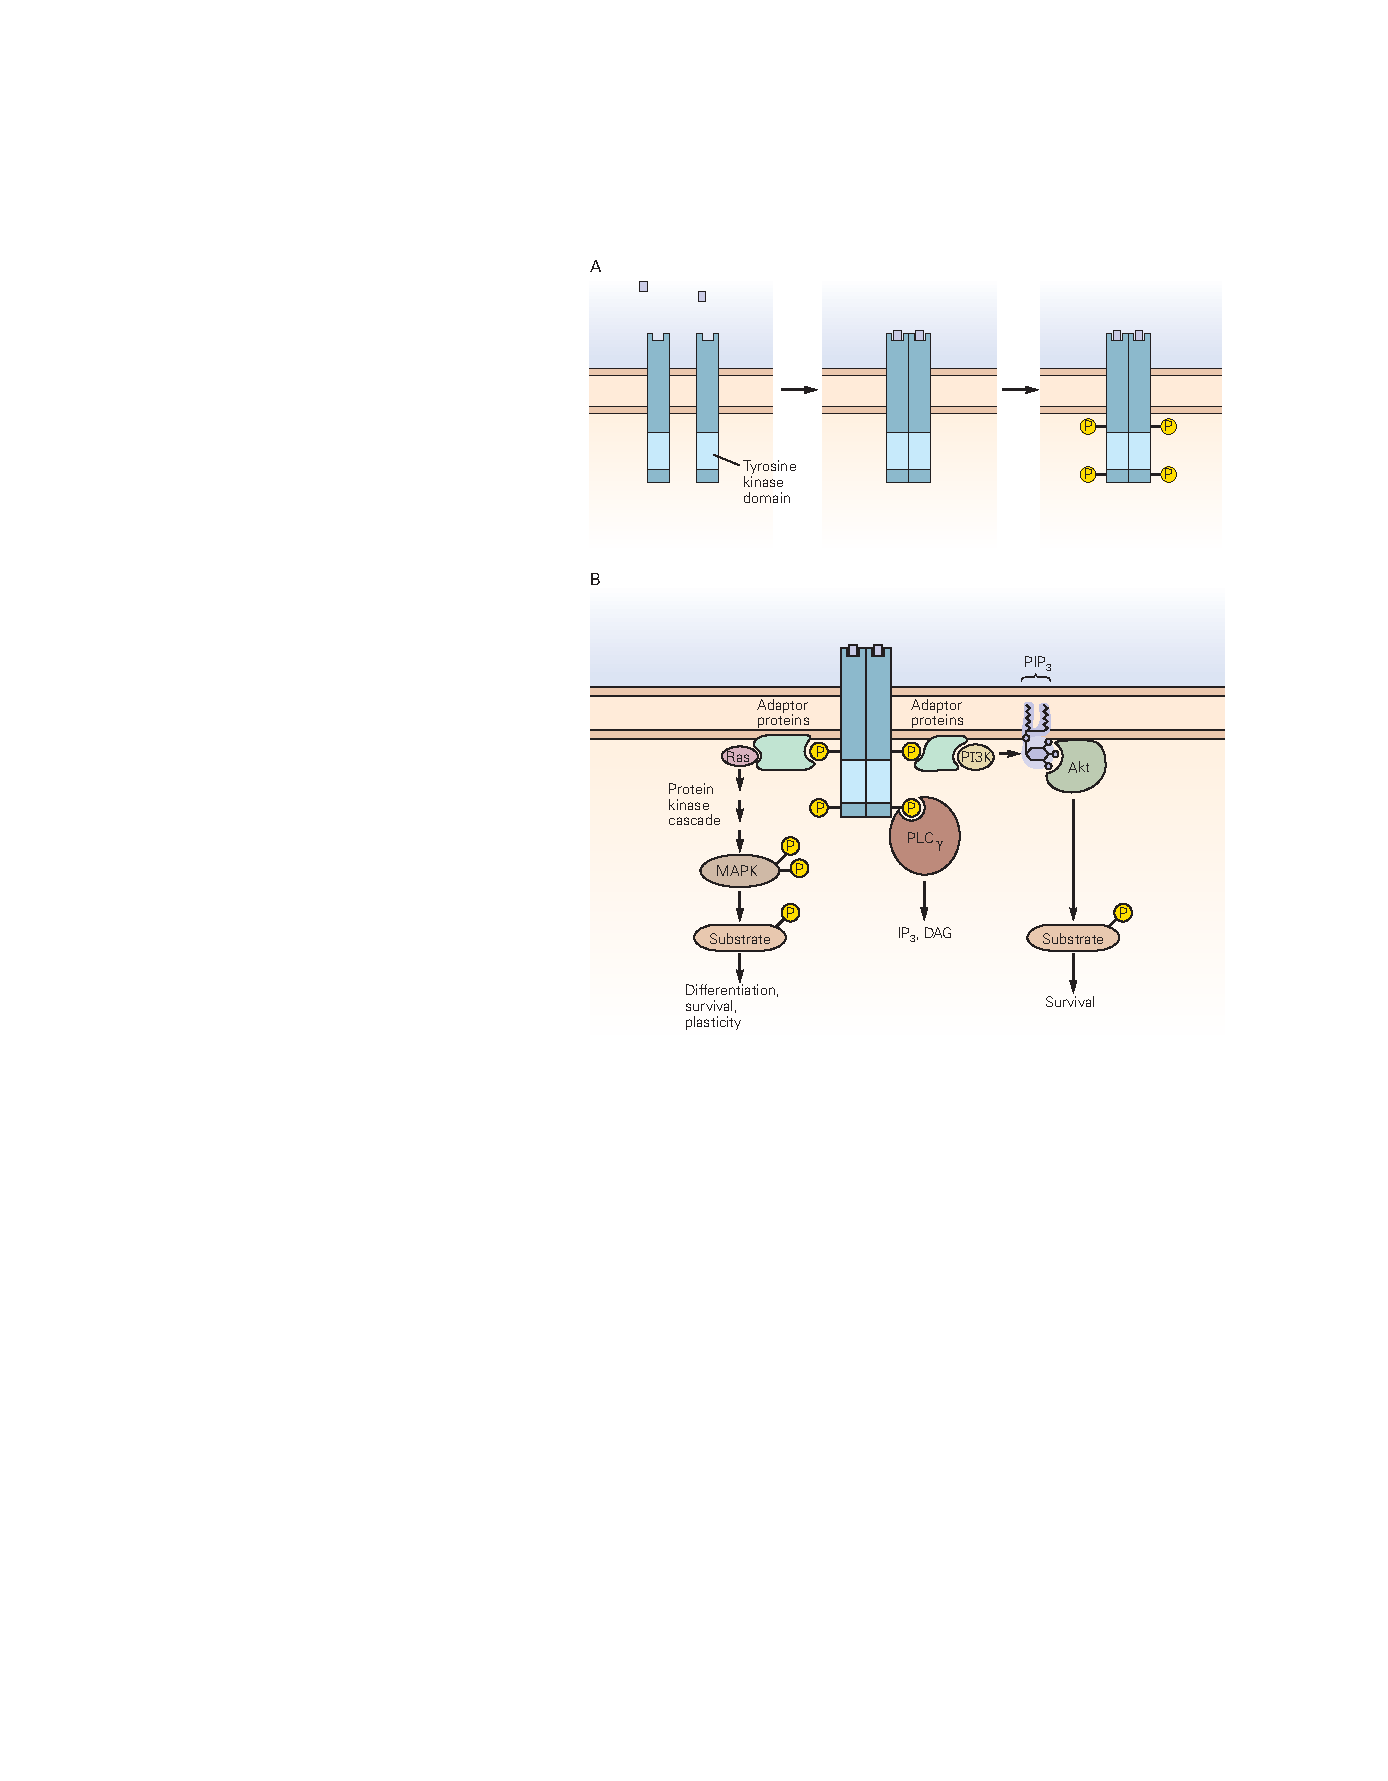
\includegraphics[width=0.7\linewidth]{chap14/fig_14_5}
	\caption{受体酪氨酸激酶。 
		\textbf{A.} 受体酪氨酸激酶在没有配体的情况下是单体。
		该受体包含一个大的细胞外结合域,该域通过单个跨膜片段连接到一个包含催化酪氨酸激酶域的大细胞内区域。
		与受体结合的配体通常会导致两个受体亚基形成二聚体,使酶能够在膜细胞质侧的各种酪氨酸残基上磷酸化自身。
		\textbf{B.} 受体自磷酸化后,一些下游信号级联通过特定接头蛋白与受体磷酸酪氨酸残基 (P) 的结合而被激活。
		左图:\textit{有丝分裂原活化蛋白激酶}的激活。
		一系列衔接蛋白募集小\textit{三磷酸鸟苷}结合蛋白 Ras,激活蛋白激酶级联,导致附近苏氨酸和酪氨酸残基上的 MAP 激酶双重磷酸化。
		激活的 MAP 激酶然后磷酸化丝氨酸和苏氨酸残基上的底物蛋白,包括离子通道和转录因子。
		中:磷脂酶 C$\gamma$ (PLC$\gamma$) 在与不同的磷酸酪氨酸残基结合时被激活,提供了一种不依赖于 G 蛋白的\textit{肌醇1,4,5-三磷酸}和甘油二酯 (DAG) 的产生机制。
		右图:Akt 蛋白激酶(也称为 PKB)的激活。
		衔接蛋白首先激活磷酸肌醇 3-激酶 (PI3K),它向 PIP2 添加一个磷酸基团,产生 PIP3,然后激活 Akt。}
	\label{fig:14_5}
\end{figure}


受体酪氨酸激酶在与肽激素结合时被激活,这些肽激素包括表皮生长因子 (EGF)、成纤维细胞生长因子 (FGF)、神经生长因子 (NGF)、脑源性神经营养因子 (BDNF) 和胰岛素。
细胞还含有重要的非受体细胞质酪氨酸激酶,例如原癌基因 src。
这些非受体酪氨酸激酶通常通过与受体酪氨酸激酶的相互作用而被激活,并且在调节生长和发育方面很重要。


许多(但不是全部)受体酪氨酸激酶在没有配体的情况下以单体形式存在于质膜中。
配体结合导致两个单体受体亚基形成二聚体,从而激活细胞内激酶。
每个单体在酪氨酸残基处磷酸化其对应物,这一作用使激酶能够磷酸化其他蛋白质。
与丝氨酸和苏氨酸蛋白激酶一样,酪氨酸激酶调节它们磷酸化的神经元蛋白的活性,包括某些离子通道的活性。
酪氨酸激酶还激活磷脂酶 C 的同种型磷脂酶 C$\gamma$,它像 PLC$\beta$ 一样将 PIP2 切割成\textit{肌醇1,4,5-三磷酸}和 DAG。


受体酪氨酸激酶启动级联反应,涉及几种衔接蛋白和其他蛋白激酶,这些蛋白激酶通常会导致基因转录发生变化。 丝裂原活化蛋白激酶 (MAP 激酶) 是一组重要的丝氨酸-苏氨酸激酶,可被受体酪氨酸激酶启动的信号级联激活。
MAP 激酶被级联的蛋白激酶反应(激酶激酶)激活,每个级联特定于三种类型的 MAP 激酶之一:细胞外信号调节激酶 (ERK)、p38 MAP 激酶和 c-Jun N-末端激酶( JNK)。
活化的 MAP 激酶有几个重要的作用。
它们易位到细胞核,在那里它们通过磷酸化某些转录因子来开启基因转录。
这一行动被认为对稳定长期记忆的形成很重要(第 ~\ref{chap:chap53}~和~\ref{chap:chap54}~章)。
MAP 激酶还磷酸化细胞质和膜蛋白以产生短期调节作用(图~\ref{fig:14_5}B)。



\section{几类代谢物可以作为跨细胞信使}

到目前为止,我们考虑的对\textit{代谢型受体}作用作出反应的代谢产物不容易穿过细胞膜。
因此,它们充当真正的细胞内第二信使:
它们只影响产生它们的细胞。
然而,细胞也可以合成脂溶性代谢物,因此既可以作用于产生它们的细胞,也可以扩散穿过质膜影响邻近细胞。
我们将此类分子称为跨细胞信使。


尽管这些分子在功能上与神经递质有一些相似之处,但它们在许多重要方面有所不同。
它们不包含在囊泡中,也不在专门的突触接触处释放。
它们通常不作用于膜受体,而是穿过邻近细胞的质膜到达细胞内靶点。
而且它们的释放和动作比快速突触处的要慢得多。
我们将考虑三大类跨细胞信使:
脂质分子花生四烯酸、内源性大麻素和气体一氧化氮的环氧合酶和脂氧合酶代谢物。



\subsection{磷脂酶 A2 水解磷脂释放花生四烯酸以产生其他第二信使}

磷脂酶 A2 水解不同于 PIP2 的磷脂,裂解甘油骨架 2' 位与花生四烯酸之间的脂肪酰基键。
这会释放花生四烯酸,然后通过酶促作用将其转化为称为类花生酸的活性代谢物家族之一,因其具有 20 个(希腊语 eicosa)碳原子而得名。


三类酶代谢花生四烯酸:
(1)环氧合酶,产生前列腺素和血栓素;
(2) 几种脂氧合酶,产生多种其他代谢产物;
(3) 细胞色素 P450 复合物,它氧化花生四烯酸本身以及环氧合酶和脂肪氧化酶代谢物(图~\ref{fig:14_6})。
大脑中前列腺素和血栓烷的合成会因非特异性刺激而显着增加,例如电休克、创伤或急性脑缺血(局部血流缺失)。
这些代谢物都可以由合成它们的细胞释放,从而充当跨细胞信号。
前列腺素的许多作用是通过在质膜上作用于 G 蛋白偶联受体家族来介导的。
该受体家族的成员可以依次激活或抑制腺苷酸环化酶或激活磷脂酶 C。


\begin{figure}[htbp]
	\centering
	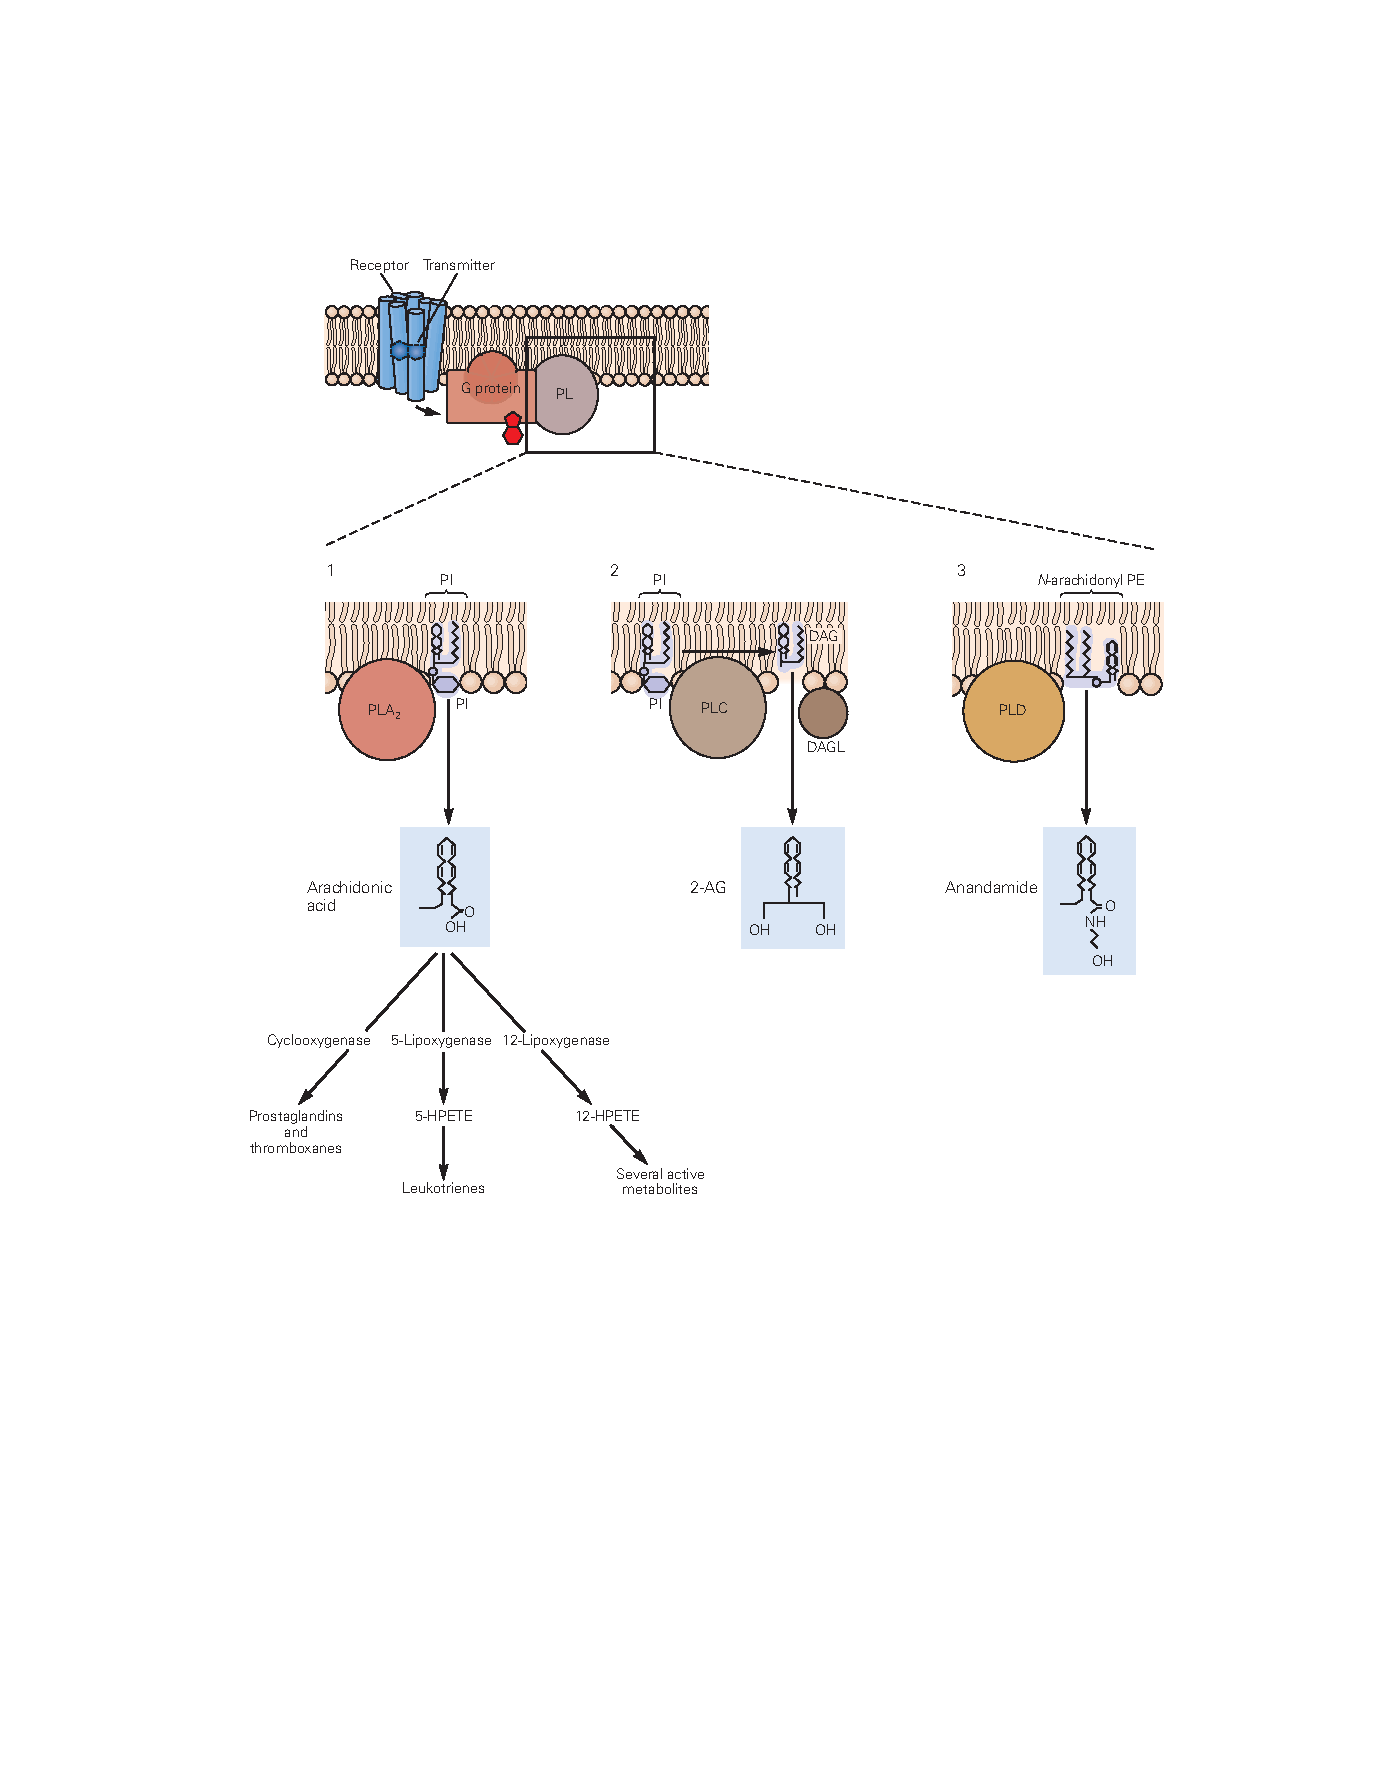
\includegraphics[width=0.8\linewidth]{chap14/fig_14_6}
	\caption{三种磷脂酶通过水解含有花生四烯酸的磷脂产生不同的第二信使。
		途径 1. 刺激 G 蛋白偶联受体导致游离 $\beta \gamma$-亚基复合物激活磷脂酶 A2 (PLA2)。
		磷脂酶 A2 水解质膜中的磷脂酰肌醇 (PI),导致释放花生四烯酸,这是一种具有四个双键的 20 碳脂肪酸,是许多磷脂的组成部分。
		一旦释放,花生四烯酸就会通过几种途径代谢,图中显示了其中三种。
		12- 和 5- 脂肪氧化酶途径均产生多种活性代谢物;
		环氧合酶途径产生前列腺素和血栓素。
		环氧合酶被吲哚美辛、阿司匹林和其他非甾体类抗炎药抑制。
		花生四烯酸及其许多代谢物调节某些离子通道的活性。
		(HPETE,氢过氧二十碳四烯酸。)途径 2。
		其他 G 蛋白激活磷脂酶 C (PLC),后者水解膜中的 PI 生成 DAG(见图~\ref{fig:14_4}。
		第二种酶二酰基甘油脂肪酶 (DAGL) 水解 DAG,导致产生 2-花生四烯基甘油 (2-AG),这是一种从神经元膜释放的内源性大麻素,然后激活其他细胞质膜中的 G 蛋白偶联内源性大麻素受体 相邻的神经元。
		途径 3. 细胞内 \ce{Ca^2+} 升高激活磷脂酶 D (PLD),后者水解具有异常极性头基的磷脂,其中含有花生四烯酸(N-花生四烯基磷脂酰乙醇胺 [N-花生四烯基 PE])。
		该作用会产生第二种内源性大麻素,称为 anandamide(花生四烯基乙醇酰胺)。}
	\label{fig:14_6}
\end{figure}



\subsection{内源性大麻素是抑制突触前递质释放的跨细胞信使}

在 1990 年代初期,研究人员发现了两种类型的 G 蛋白偶联受体 CB1 和 CB2,它们以高亲和力结合大麻中的活性化合物 Δ9-四氢大麻酚 (THC)。
这两类受体都与 G 蛋白的 Gi 和 Go 类型偶联。
CB1 受体是大脑中最丰富的 G 蛋白偶联受体类型,主要存在于中枢和周围神经系统的轴突和突触前末梢。
这些受体的激活会抑制多种神经递质的释放,包括 GABA 和谷氨酸。
CB2 受体主要存在于淋巴细胞上,在那里它们调节免疫反应。


大麻素受体的鉴定导致其内源性配体,内源性大麻素的纯化。
已经确定了两种主要的内源性大麻素;
两者均含有花生四烯酸部分并结合 CB1 和 CB2 受体。 
花生四烯酸(梵文ananda,bliss)由花生四烯酸与乙醇胺(花生四烯基乙醇胺)偶联而成;
2-花生四烯基甘油 (2-AG) 由在甘油 2 位酯化的花生四烯酸组成。
两者均由含有花生四烯酸的磷脂酶促水解产生,该过程在某些 G 蛋白偶联受体受到刺激或内部 \ce{Ca^2+} 浓度升高时启动(图 14-6)。
然而,虽然 2-AG 在几乎所有神经元中合成,但 anandamide 的来源不太清楚。


因为内源性大麻素是可以通过膜扩散的脂质代谢物,所以它们起到跨细胞信号的作用,作用于邻近细胞,包括突触前末梢。
这些代谢物的产生通常在突触后神经元中受到突触后兴奋引起的细胞内 \ce{Ca^2+} 增加的刺激。
一旦产生,内源性大麻素就会通过细胞膜扩散到附近的突触前末端,在那里它们与 CB1 受体结合并抑制递质释放。
以这种方式,突触后细胞可以控制突触前神经元的活动。 
现在人们对了解大脑中这些受体的激活如何导致大麻的各种行为影响产生了浓厚的兴趣。



\subsection{气态第二信使\textit{一氧化氮}是一种刺激环\textit{鸟苷-3,5-单磷酸盐}合成的跨细胞信号}

\textit{一氧化氮}在神经元和身体其他细胞中充当跨细胞信使。
\textit{一氧化氮}的调节功能是通过其作为从血管内皮细胞释放的局部激素的作用而发现的,导致血管壁平滑肌松弛。
与花生四烯酸的代谢物一样,\textit{一氧化氮}很容易穿过细胞膜,并且可以影响附近的细胞而不作用于表面受体。
一氧化氮是一种自由基,因此具有高反应性和短寿命。


一氧化氮通过刺激\textit{环鸟苷-3,5-单磷酸盐}的合成产生许多作用,它与\textit{环磷酸腺苷}一样是激活蛋白激酶的细胞质第二信使。
具体来说,\textit{一氧化氮}激活鸟苷酸环化酶,该酶将\textit{三磷酸鸟苷}转化为\textit{环鸟苷-3,5-单磷酸盐}。
有两种类型的鸟苷酸环化酶。 
一种是完整的膜蛋白,具有细胞外受体结构域和合成\textit{环鸟苷-3,5-单磷酸盐}的细胞内催化结构域。
另一种是细胞质的(可溶性鸟苷酸环化酶),是被\textit{一氧化氮}激活的亚型。
在某些情况下,\textit{一氧化氮}被认为通过修饰各种蛋白质的半胱氨酸残基上的巯基而直接起作用,这一过程称为亚硝基化。


循环 GMP 有两个主要作用。
它直接作用于打开环核苷酸门控通道(对光转导和嗅觉信号很重要,分别在第~\ref{chap:chap22}~章和第~\ref{chap:chap29}~章中描述),并激活\textit{环鸟苷-3,5-单磷酸盐}依赖性蛋白激酶 (PKG),它像\textit{蛋白激酶A}一样磷酸化某些底物蛋白 丝氨酸或苏氨酸残基。
PKG 与\textit{蛋白激酶A}的不同之处在于它是具有调节(\textit{环鸟苷-3,5-单磷酸盐}结合)和催化结构域的单一多肽,与其他蛋白激酶中的调节和催化结构域同源。
它还磷酸化一组与\textit{蛋白激酶A}不同的底物。


循环 GMP 依赖性蛋白质磷酸化在小脑的浦肯野细胞、具有大量分支树突的大神经元中很突出。
在那里,\textit{环鸟苷-3,5-单磷酸盐}级联由颗粒细胞轴突(平行纤维)的突触前末端产生和释放的\textit{一氧化氮}激活,这些轴突在浦肯野细胞上形成兴奋性突触。
浦肯野神经元中\textit{环鸟苷-3,5-单磷酸盐}的增加降低了 AMPA 受体对谷氨酸的反应,从而抑制了平行纤维突触的快速兴奋性传递。



\section{代谢型受体的生理作用不同于离子型受体}

\subsection{第二信使级联可以增加或减少多种离子通道的开放}

代谢型和离子型受体之间的功能差异反映了它们特性的差异。
例如,代谢型受体作用比离子型受体作用慢得多(表 14-1)。
两类受体的生理作用也不同。


离子型受体是起简单开关作用的通道;
它们的主要工作是要么激发神经元使其更接近放电阈值,要么抑制神经元以降低其放电的可能性。
因为这些通道通常局限于膜的突触后区域,所以离子型受体的作用是局部的。
另一方面,代谢型受体因为它们激活可扩散的第二信使,可以作用于距受体一定距离的通道。
此外,代谢受体调节多种通道类型,包括静息通道、配体门控通道和产生动作电位的电压门控通道,构成起搏器电位的基础,并为神经递质释放提供 \ce{Ca^2+} 流入。


最后,虽然递质结合导致离子型受体通道开放增加,但代谢型受体的激活可导致通道开放增加或减少。
例如,海马锥体神经元树突中失活(A 型)\ce{K+} 通道的 MAP 激酶磷酸化会减少通道开放,从而减少 \ce{K+} 电流幅度,从而增强树突动作电位放电。


递质与代谢受体的结合可以极大地影响神经元的电生理特性(图~\ref{fig:14_7})。
突触前末端的代谢型受体可以通过调节 \ce{Ca^2+} 流入或突触释放过程本身的功效来改变递质释放(图~\ref{fig:14_7}A)。
突触后细胞中的代谢型受体可以通过调节介导突触后电位的离子型受体来影响突触的强度(图~\ref{fig:14_7} B)。
通过作用于突触后神经元细胞体、树突和轴突中的静息和电压门控通道,\textit{代谢型受体}的作用还可以改变静息电位、膜电阻、长度和时间常数、阈值电位、动作电位持续时间和重复放电特性。
这种对神经元内在兴奋性的调节可以在调节通过神经元回路的信息流以改变行为方面发挥重要作用。


\begin{figure}[htbp]
	\centering
	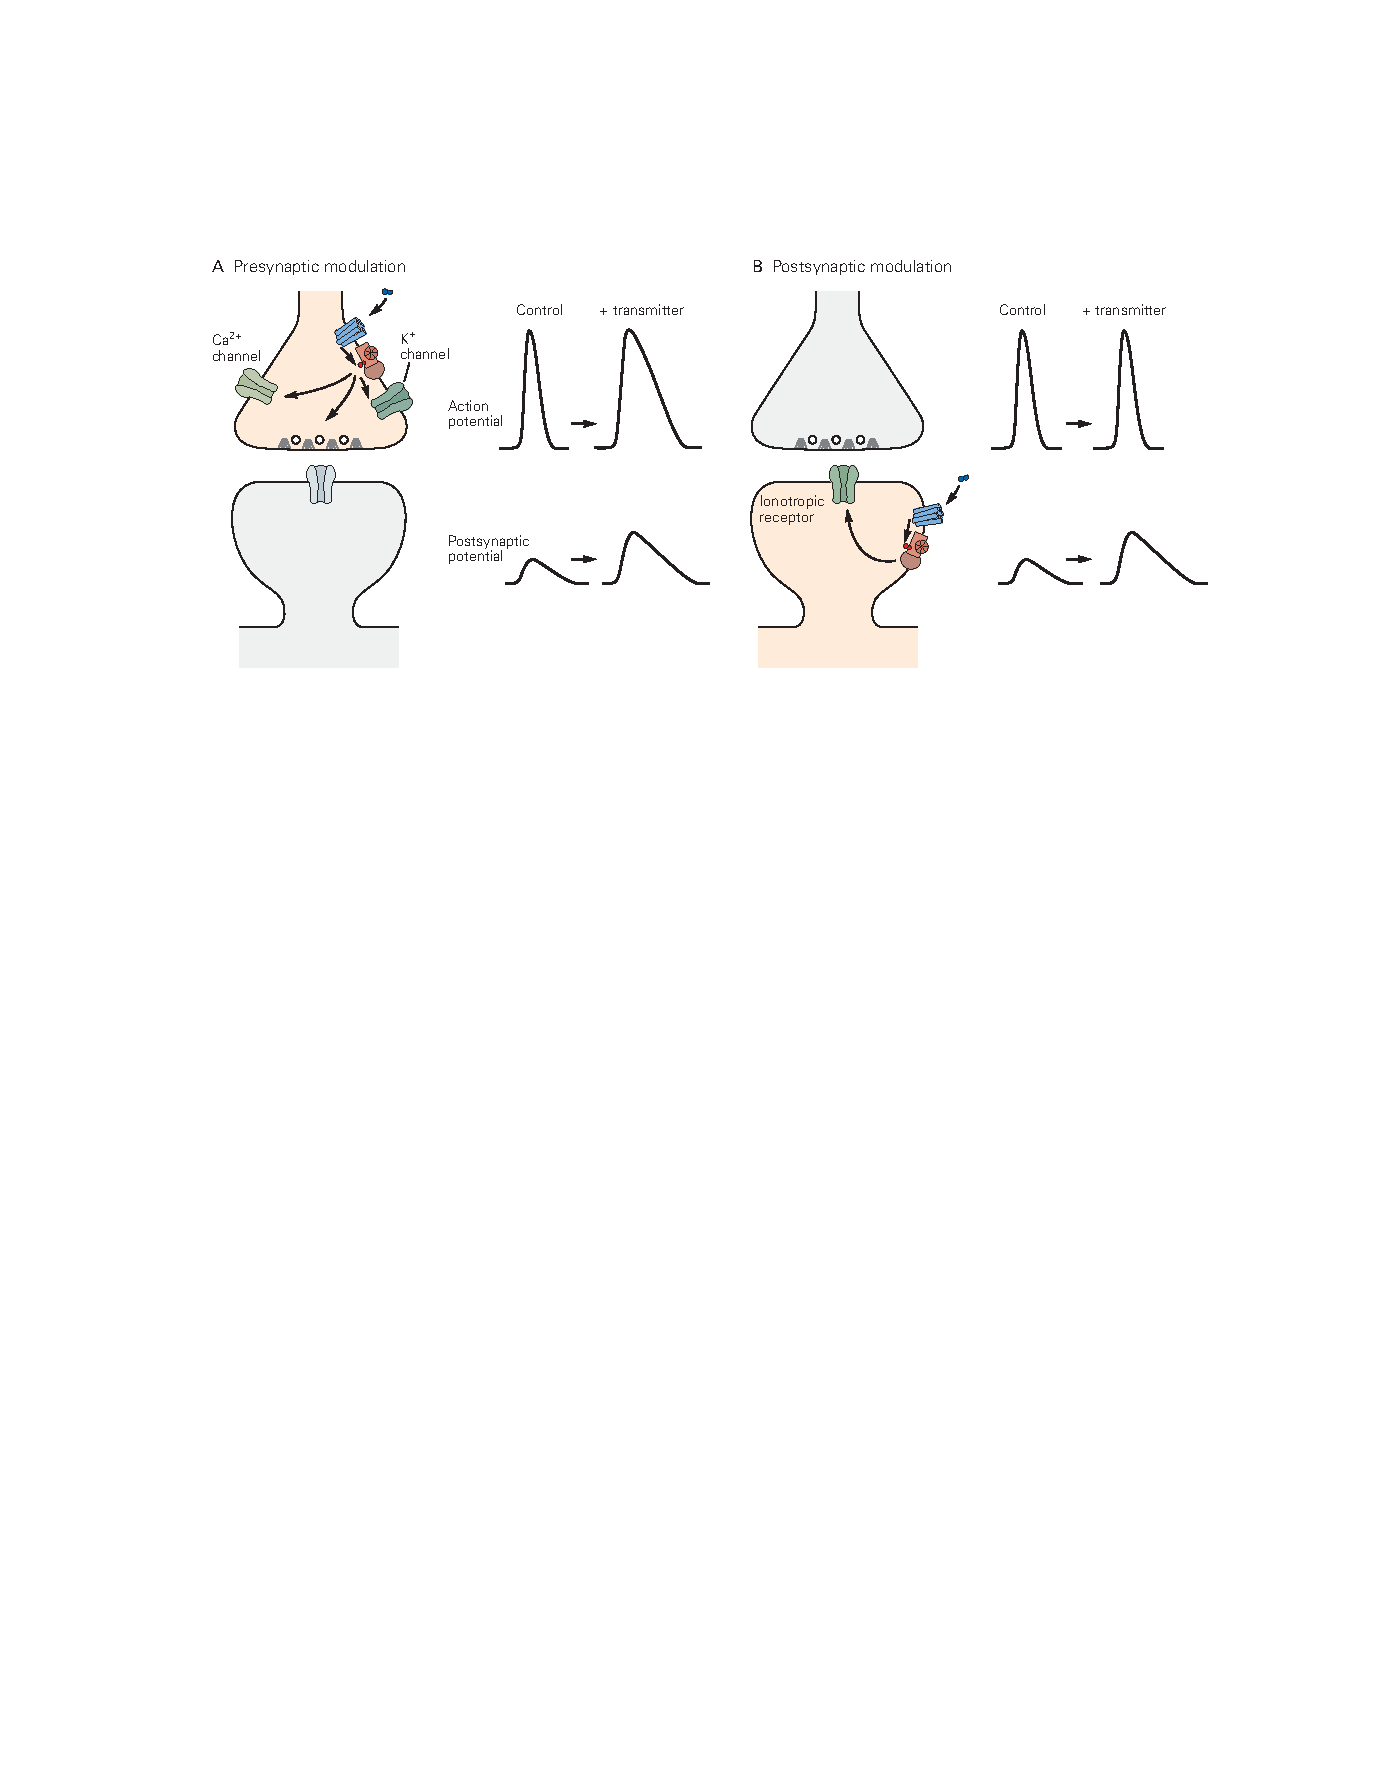
\includegraphics[width=0.9\linewidth]{chap14/fig_14_7}
	\caption{第二信使的调节作用可以通过作用于两个突触位点来调节快速突触传递。 A. 在突触前末梢,第二信使可以调节递质释放的功效,从而调节由离子型受体介导的快速突触后电位的大小。 这可以通过改变突触前 Ca2+ 流入来发生,直接通过调节突触前电压门控 \ce{Ca^2+} 通道或间接通过调节突触前 \ce{K+} 通道,通过控制动作电位持续时间来改变 \ce{Ca^2+} 流入(如图所示,从而改变 \ce{Ca^2+} 通道保持开放的时间长度) . 一些调制发射器直接调节释放机制的功效。 B. 在突触后末梢,第二信使可以通过调节离子型受体直接改变突触后电位的幅度。}
	\label{fig:14_7}
\end{figure}


周围神经系统自主神经节中的胆碱能突触传递很好地说明了离子通道的直接和间接调节之间的区别。
刺激突触前神经从神经末梢释放\textit{乙酰胆碱},直接打开突触后神经元中的烟碱\textit{乙酰胆碱}受体通道,从而产生快速\textit{兴奋性突触后电位}。
快速\textit{兴奋性突触后电位}之后是慢速\textit{兴奋性突触后电位},大约需要 100 毫秒才能发展,但随后会持续几秒钟。
缓慢的\textit{兴奋性突触后电位}由\textit{乙酰胆碱}对代谢型毒蕈碱受体的作用产生,导致延迟整流 \ce{K+} 通道关闭,称为毒蕈碱敏感(或 M 型)\ce{K+} 通道(图~\ref{fig:14_8} A)。
这些由 KCNQ 基因家族成员形成的电压门控通道在细胞静止时被部分激活;
因此,它们携带的电流有助于确定细胞静息电位和膜电阻。


\begin{figure}[htbp]
	\centering
	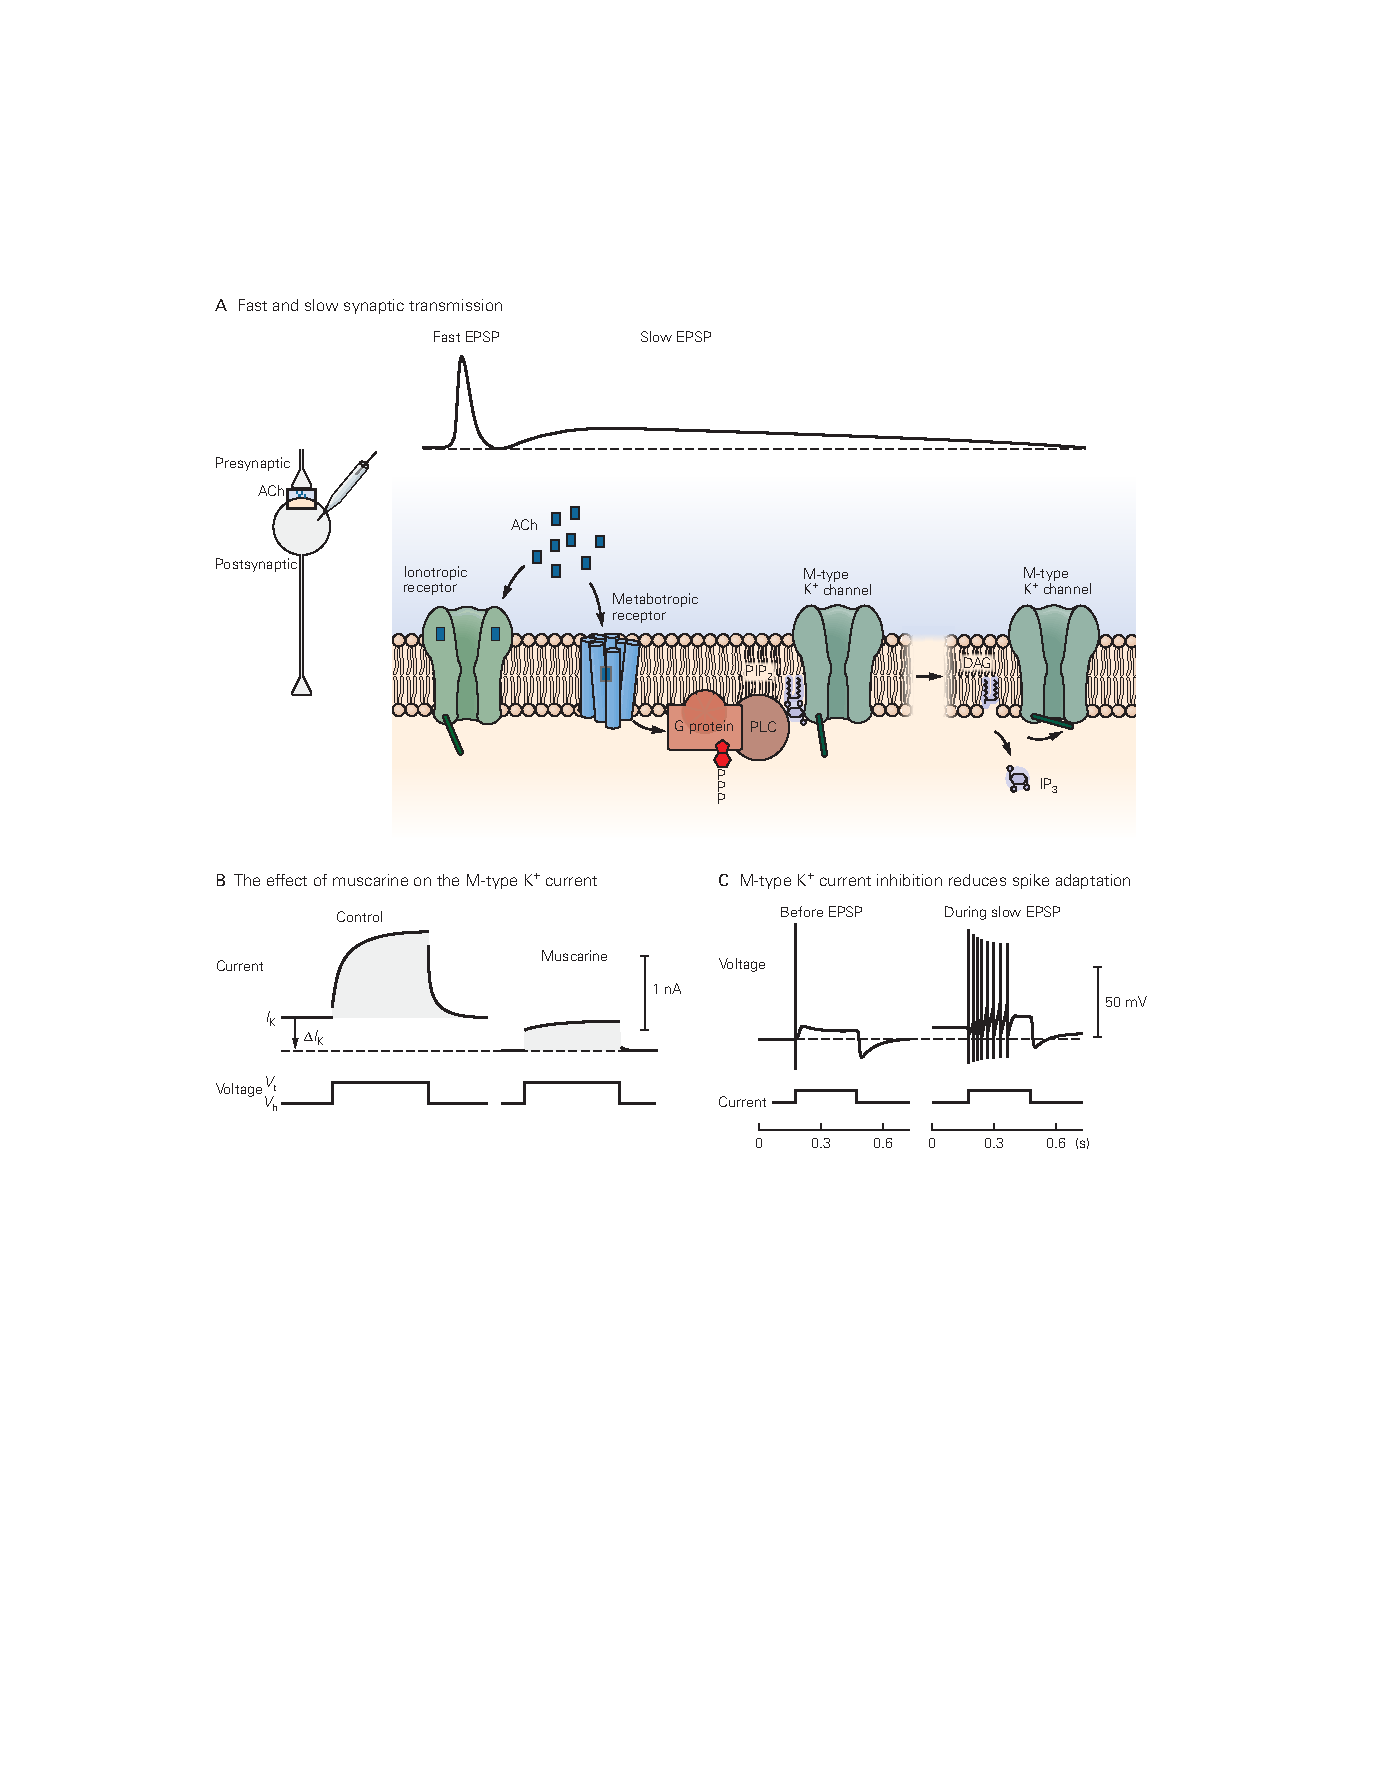
\includegraphics[width=0.8\linewidth]{chap14/fig_14_8}
	\caption{自主神经节的快速离子型和慢速代谢型突触动作。
		\textbf{A.} \textit{乙酰胆碱}释放到自主神经节的突触后神经元上会产生一个快速的\textit{兴奋性突触后电位},然后是一个缓慢的\textit{兴奋性突触后电位}。
		快速\textit{兴奋性突触后电位}由离子型烟碱\textit{乙酰胆碱}受体激活产生,慢 EPSP 由代谢型毒蕈碱\textit{乙酰胆碱}受体激活产生。
		\textit{代谢型受体}刺激 PLC 水解 PIP2,产生\textit{肌醇1,4,5-三磷酸}和 DAG。 PIP2 的减少导致 M 型延迟整流 \ce{K+} 通道关闭。
		\textbf{B.} 来自自主神经节神经元的电压钳记录表明\textit{乙酰胆碱}降低了电压门控 M 型 \ce{K+} 通道携带的电流幅度。
		在这个实验中,细胞最初被钳制在一个接近静息电位的保持电位 (Vh),在没有\textit{乙酰胆碱}的情况下(通常为 –60 毫伏)。
		在此电位下,M 型 \ce{K+} 通道部分打开,导致稳定的外向 \ce{K+} 电流。
		然后将电压步进 1 秒至更正的测试电位(Vt,通常为 –40 毫伏),这通常会导致外向 \ce{K+} 电流 (IK) 缓慢增加,因为 M 型 \ce{K+} 通道对更正的电压作出响应 增加他们的开放(控制)。
		毒蕈碱(一种选择性刺激毒蕈碱\textit{乙酰胆碱}受体的植物生物碱)的应用导致部分 M 型 \ce{K+} 通道关闭。
		这通过关闭在静止状态下打开的 M 型 \ce{K+} 通道,降低了保持电位下的外向 \ce{K+} 电流(注意基线电流的变化,ΔIK),并降低了响应阶跃的缓慢激活 \ce{K+} 电流的幅度 去极化\cite{adams1986slow}。
		\textbf{C.} 在没有毒蕈碱\textit{乙酰胆碱}受体刺激的情况下,神经元仅发射一个动作电位以响应长时间的去极化电流刺激,这一过程称为尖峰频率适应(左)。
		这是因为在去极化过程中 M 型 \ce{K+} 通道的缓慢激活会产生外向电流,使膜在阈值以下重新极化。
		当在缓慢的\textit{兴奋性突触后电位}期间应用相同的电流刺激时,当大部分 M 型通道现在无法打开时,神经元会激发更持久的动作电位序列(右)\cite{adams1986slow}。}
	\label{fig:14_8}
\end{figure}


M 型 \ce{K+} 通道与其他延迟整流 \ce{K+} 通道的不同之处在于其激活速度要慢得多。
它需要几百毫秒才能完全激活去极化。
因为 M 型通道在静息电位部分开放,它们响应毒蕈碱刺激而关闭导致静息 \ce{K+} 电导降低,从而使细胞去极化(图~\ref{fig:14_8} B)。
膜将去极化多远?
这可以使用 Goldman 方程(第~\ref{chap:chap9} ~章)的等效电路形式通过从其初始值减少 gK 项来计算。
由于 M 型 \ce{K+} 通道关闭导致的 gK 变化相对较小,慢速\textit{兴奋性突触后电位}峰值处的去极化很小,只有几毫伏。
尽管如此,\textit{乙酰胆碱}关闭 M 型 \ce{K+} 通道可导致响应去极化输入的动作电位激发显着增加。


显着增强兴奋性的 M 型 \ce{K+} 通道关闭有哪些特殊性质?
首先,静息 gK 减少导致的去极化使膜更接近阈值。
其次,膜电阻的增加降低了将细胞去极化到给定电压所需的兴奋电流量。
第三,延迟 \ce{K+} 电流的减少使细胞能够产生更持久的动作电位放电,以响应延长的去极化刺激。


在没有\textit{乙酰胆碱}的情况下,神经节神经元通常只发射一个或两个动作电位,然后停止发射以响应刚好高于阈值的长时间兴奋性刺激。
这个过程称为尖峰频率适应,部分原因是 M 型 \ce{K+} 电流增加以响应延长的去极化,这有助于使膜重新极化到阈值以下。
因此,如果在缓慢的\textit{兴奋性突触后电位}期间应用相同的延长刺激(当 M 型 \ce{K+} 通道关闭时),神经元在整个刺激期间保持去极化高于阈值,从而激发长时间的脉冲爆发(图~\ref{fig:14_8}C)。
正如\textit{乙酰胆碱}的这种调节所说明的那样,M 型 \ce{K+} 通道的作用不仅仅是帮助设置静息电位——它们还控制兴奋性。


虽然一段时间以来已知自主神经节中的毒蕈碱受体作用会导致 PLC 的激活以及 DAG 和\textit{肌醇1,4,5-三磷酸}的产生,但这种信号级联产生 M 型通道关闭的确切机制仍然是个谜。
然而,现在很清楚,毒蕈碱受体激活后 M 通道关闭不是由于第二信使的产生。
相反,M 通道以及许多其他类型的通道(例如,参见图~\ref{fig:14_10})结合膜质 PIP2 作为其正常功能的辅因子。
因此,毒蕈碱受体激活通过激活 PLC 关闭 M 型通道,从而降低膜中由于 PLC 水解而导致的 PIP2 水平。
接下来我们将讨论其他信号级联能够调节其他类型离子通道的机制。
我们首先描述最简单的机制,即 G 蛋白对离子通道的直接门控,然后考虑依赖于\textit{蛋白激酶A}的蛋白质磷酸化的更复杂机制。


\begin{figure}[htbp]
	\centering
	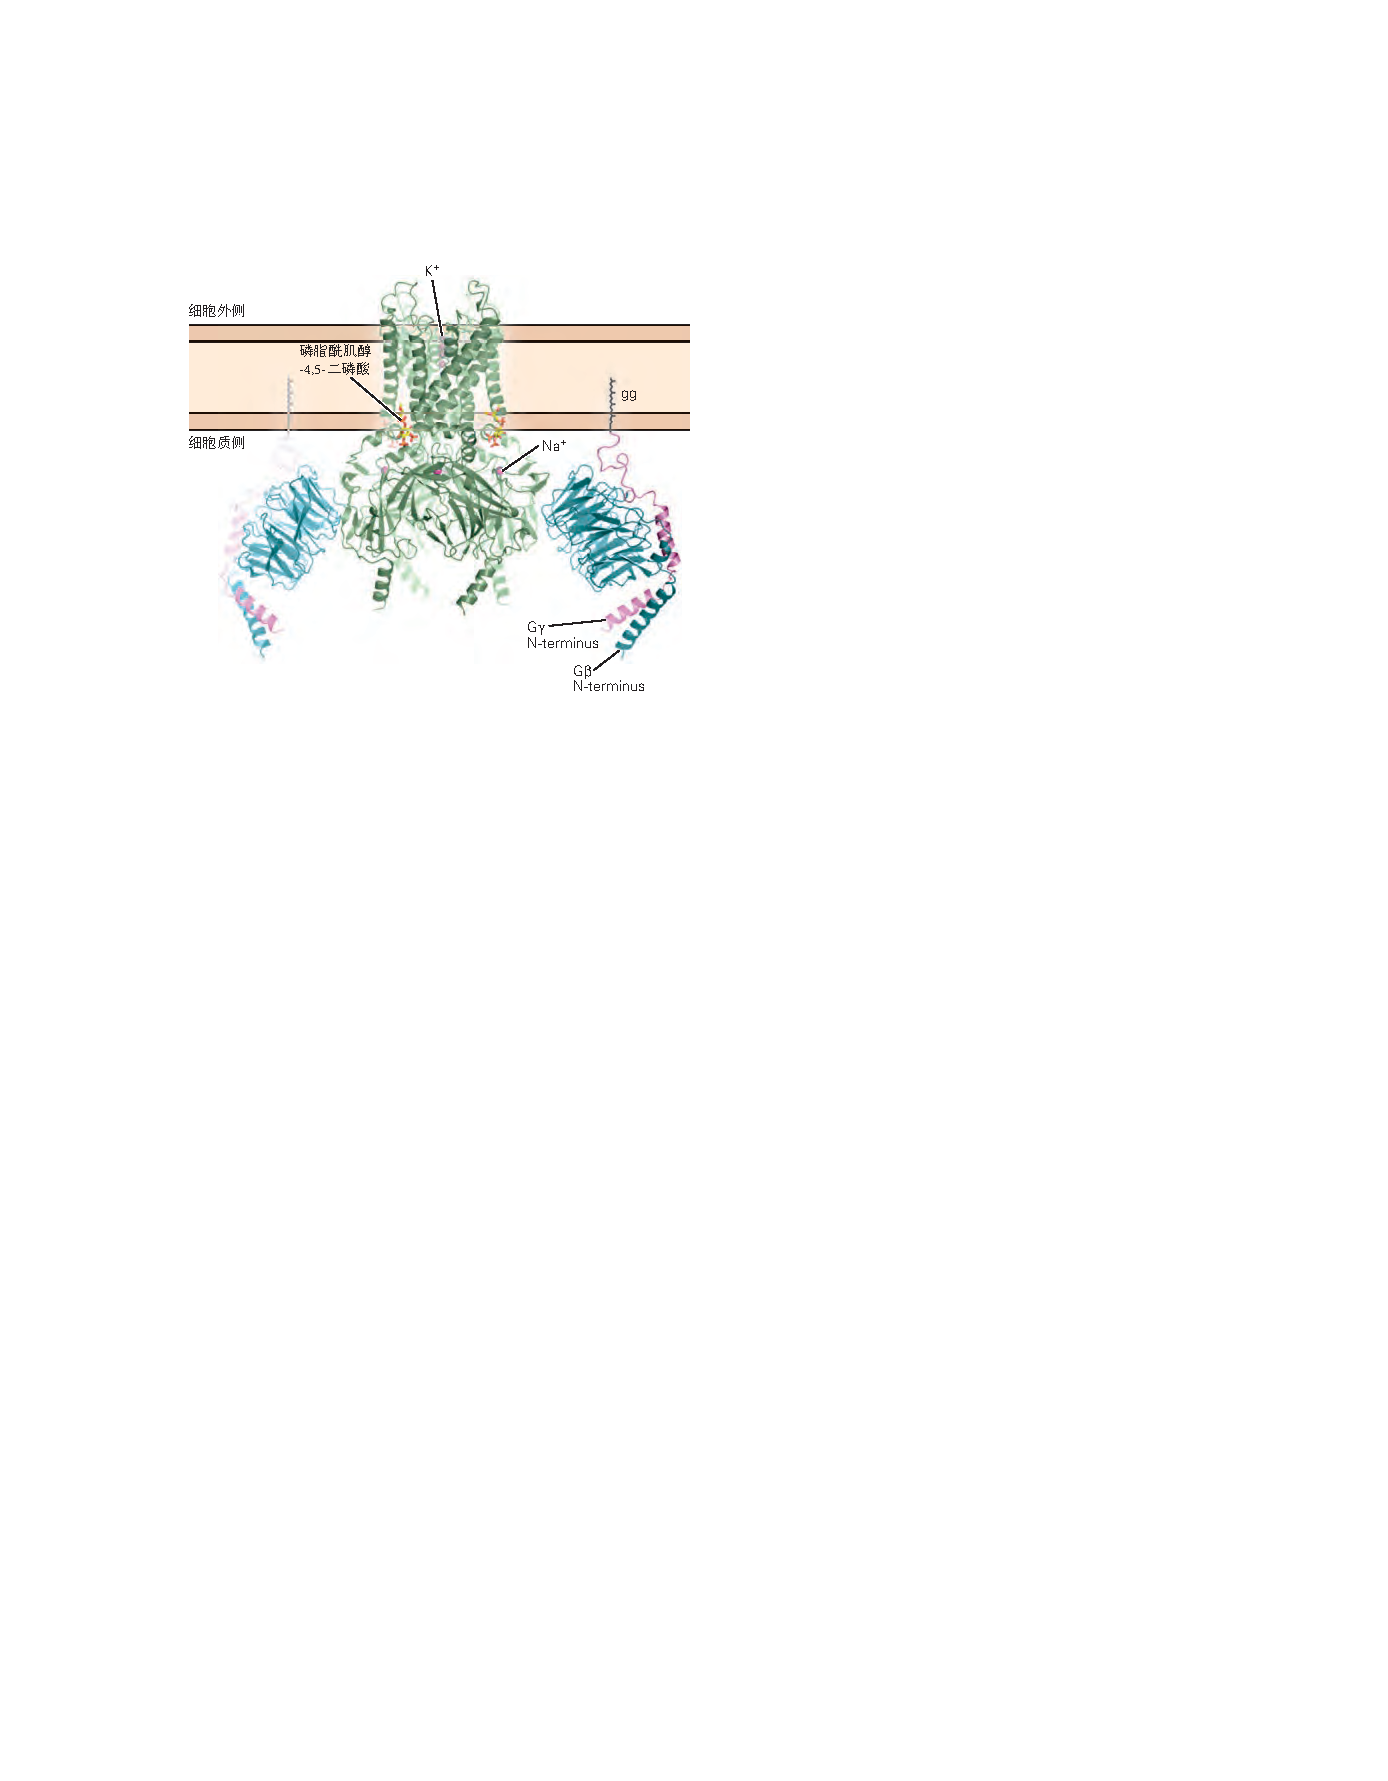
\includegraphics[width=0.5\linewidth]{chap14/fig_14_10}
	\caption{G 蛋白$\beta\gamma$亚基可直接结合并激活 GIRK 通道。
		GIRK 通道(绿色)与 G 蛋白$\beta$-亚基(G$\beta$,青色)和 $\gamma$-亚基(G$\gamma$,紫色)相互作用的高分辨率结构。
		香叶基香叶基脂质分子 (gg) 连接到 G$\gamma$ 的 C 末端。
		该结构说明 \ce{Na+} 离子和磷脂 PIP2 也与通道结合,从而增强通道开放。
		通道内的粉红色球体代表 \ce{K+} 离子\cite{whorton2013x}。}
	\label{fig:14_10}
\end{figure}



\subsection{G蛋白可以直接调节离子通道}

通道间接门控的最简单机制发生在与代谢受体结合的递质释放 G 蛋白亚基时,该亚基直接与通道相互作用以修改其开放。
该机制用于门控两种离子通道:G 蛋白门控内向整流 \ce{K+} 通道(GIRK1-4;由 KCNJ1-4 基因编码)和电压依赖性 \ce{Ca^2+} 通道。
对于这两种通道,是 G 蛋白的 $\beta \gamma$ 复合物结合并调节通道开放(图~\ref{fig:14_9} A)。


\begin{figure}[htbp]
	\centering
	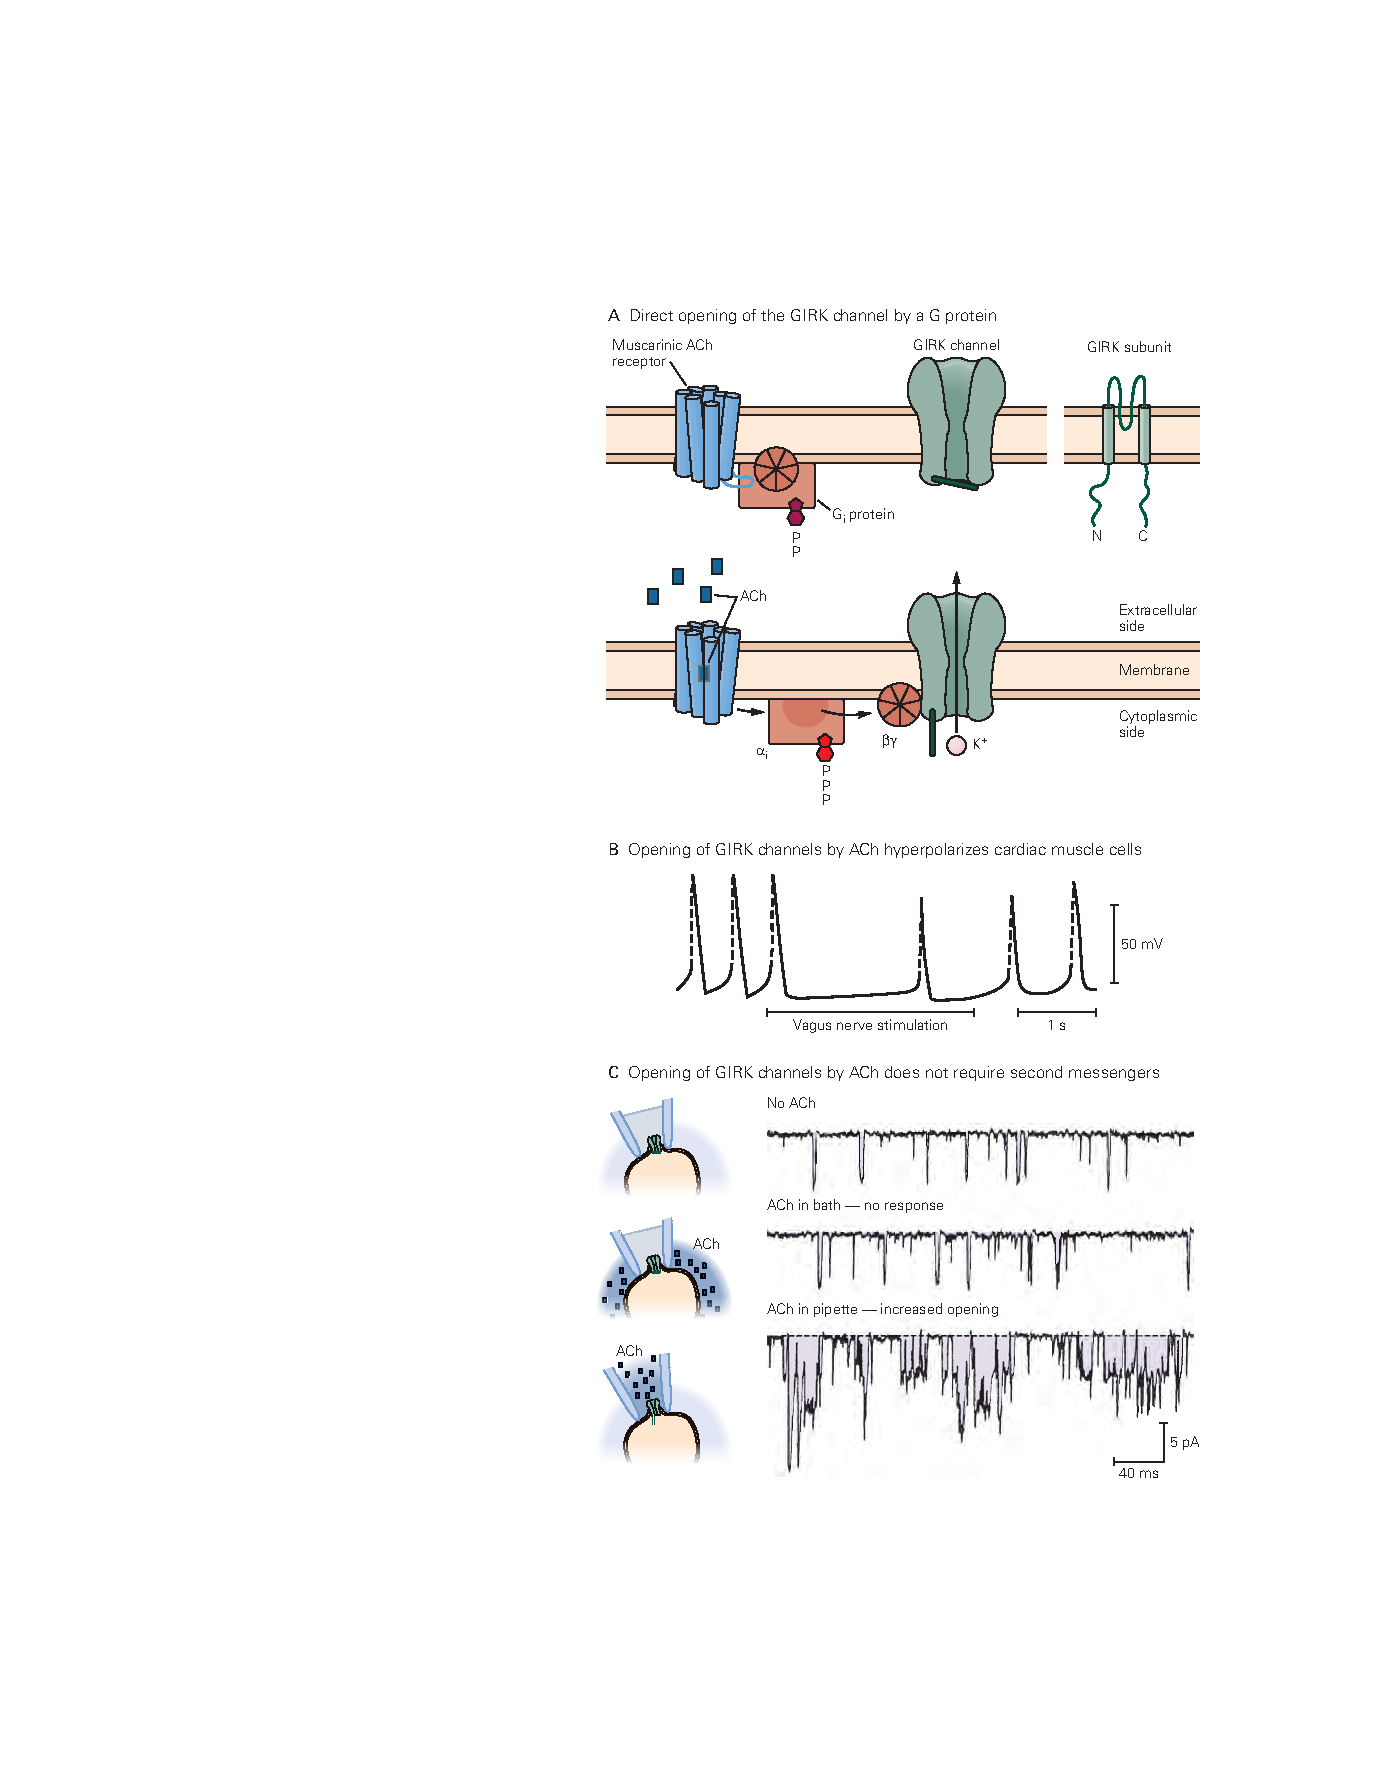
\includegraphics[width=0.65\linewidth]{chap14/fig_14_9}
	\caption{一些 G 蛋白可以直接打开离子 N C 通道,而无需使用第二信使。
		\textbf{A.} 内向整流 \ce{K+} 通道 (GIRK) 由 G 蛋白直接打开。
		\textit{乙酰胆碱}与毒蕈碱受体的结合导致 Gi 蛋白和 $\alpha$i$\beta \gamma$ 复合物解离;
		游离的 $\beta \gamma$ 亚基与通道的细胞质结构域结合,导致通道打开。
		\textbf{B.} 刺激副交感迷走神经释放\textit{乙酰胆碱},\textit{乙酰胆碱}作用于毒蕈碱受体以打开心肌细胞膜中的 GIRK 通道。
		通过 GIRK 通道的电流使细胞超极化,从而减慢心率\cite{toda1967interactions}。
		\textbf{C.} 三个单通道记录表明 GIRK 通道的打开不涉及可自由扩散的第二信使。
		在这个实验中,移液管中含有高浓度的 \ce{K+},这使得 EK 的阴性度降低。
		因此,当 GIRK 通道打开时,它们会产生短暂的内向(向下)电流脉冲。
		在没有\textit{乙酰胆碱}的情况下,通道会短暂且不频繁地打开(最高记录)。
		\textit{乙酰胆碱}在浴缸中的应用(移液器外)不会增加移液器下方膜片的通道开口(中间记录)。
		这是因为\textit{乙酰胆碱}与其受体结合释放的游离 $\beta \gamma$ 亚基仍然束缚在受体附近的膜上,只能激活附近的通道。
		亚基不能自由扩散到贴片移液器下的通道。
		\textit{乙酰胆碱}必须在移液器中才能激活通道(底部记录)\cite{soejima1984mode}。}
	\label{fig:14_9}
\end{figure}


与其他内向整流通道一样,GIRK 通道更容易向内传递电流而不是向外传递电流,尽管在生理情况下,\ce{K+} 电流总是向外传递。
内向整流器通道类似于截短的电压门控 \ce{K+} 通道,有两个跨膜区域,由 P 区环路连接,在通道中形成选择性过滤器(参见图 8-11)。


在 1920 年代,Otto Loewi 描述了\textit{乙酰胆碱}的释放如何响应迷走神经的刺激而减慢心率(图~\ref{fig:14_9} B)。
我们现在知道\textit{乙酰胆碱}激活毒蕈碱受体以刺激 G 蛋白活性,从而直接打开 GIRK 通道。
多年来,这种递质作用一直令人费解,因为它具有离子型和代谢型受体作用的特性。
\textit{乙酰胆碱}释放后激活 \ce{K+} 电流的时间进程(50 至 100 毫秒上升时间)比离子型受体(上升时间 <1 毫秒)慢。
然而,GIRK 通道的激活速率比依赖于蛋白质磷酸化的第二信使介导的作用(可能需要很多秒才能启动)快得多。 
尽管生化和电生理学研究清楚地表明该作用需要 G 蛋白,但膜片钳实验表明 G 蛋白不会触发可扩散第二信使的产生(图~\ref{fig:14_9} C)。
当发现 GIRK 通道直接被 G 蛋白的 $\beta \gamma$-亚基复合物激活时,这些发现得到了调和,当它在毒蕈碱受体激活后与 G 蛋白 $\alpha$-亚基解离时,GIRK 通道可与 GIRK 通道相互作用。


$\beta \gamma$-亚基激活 GIRK 通道的机制最近通过解析 GIRK 通道与 $\beta \gamma$-亚基复合物中的 X 射线晶体结构,在原子分辨率下得以阐明。
四个 GIRK 通道亚基中的每一个都结合一个单一的 $\beta \gamma$-亚基复合物,该复合物与通道的细胞质表面相互作用,导致促进通道开放的构象变化(图~\ref{fig:14_10})。


GIRK 通道的激活使膜在 EK (–80 毫伏) 方向超极化。 
在某些类别的自发活跃的神经元中,通过这些通道的外向 \ce{K+} 电流主要用于降低神经元的内在放电率,对抗由超极化激活的环核苷酸调节通道携带的兴奋性起搏器电流引起的缓慢去极化,这些通道被编码 由 HCN 基因家族(第~\ref{chap:chap10}~章)。
由于 GIRK 通道由神经递质激活,因此它们提供了一种突触调节可兴奋细胞放电率的方法。
这些通道在多种神经元中受到大量递质和神经肽的调节,这些递质和神经肽作用于不同的 G 蛋白偶联受体以激活 Gi 或 Go,从而释放 $\beta \gamma$ 亚基。


几种 G 蛋白偶联受体也可抑制某些电压门控 \ce{Ca^2+} 通道的开放,这也是 Gi 或 Go 的 $\beta \gamma$ 复合物与通道直接结合的结果。
因为通过电压门控 \ce{Ca^2+} 通道的 \ce{Ca^2+} 流入通常具有去极化作用,所以 G 蛋白 $\beta \gamma$-亚基的双重作用——\ce{Ca^2+} 通道抑制和 \ce{K+} 通道激活——强烈抑制神经元放电。
正如我们将在第~\ref{chap:chap15}~章中看到的那样,抑制突触前末梢的电压门控 \ce{Ca^2+} 通道可以抑制神经递质的释放。



\subsection{\textit{环磷酸腺苷}依赖性蛋白质磷酸化可以关闭钾通道}

在海洋软体动物 Aplysia 中,一组机械感受器感觉神经元通过与运动神经元的快速兴奋性突触启动防御性退缩反射以响应触觉刺激。
某些中间神经元与这些感觉神经元形成血清素能突触,中间神经元释放的血清素使退缩反射敏感,增强动物对刺激的反应,从而产生一种简单的学习形式(第~\ref{chap:chap53}~章)。


5-羟色胺的调节作用取决于它与激活 $ G_s $ 蛋白的 G 蛋白偶联受体的结合,$ G_s $ 蛋白升高\textit{环磷酸腺苷},从而激活\textit{蛋白激酶A}。
这导致直接磷酸化并随后关闭充当静息通道的 5-羟色胺敏感(或 S 型)\ce{K+} 通道(图~\ref{fig:14_11})。
与\textit{乙酰胆碱}关闭 M 型 \ce{K+} 通道一样,关闭 S 型 \ce{K+} 通道会减少细胞中的 \ce{K+} 流出,从而使细胞去极化并降低其静息膜电导。
相反,神经肽 FMRFamide 可通过花生四烯酸的 12-脂氧合酶代谢物起作用,从而增强相同 S 型 \ce{K+} 通道的开放。
这种增强的通道开放导致与静息膜电导增加相关的缓慢超极化\textit{抑制性突触后电位}。


\begin{figure}[htbp]
	\centering
	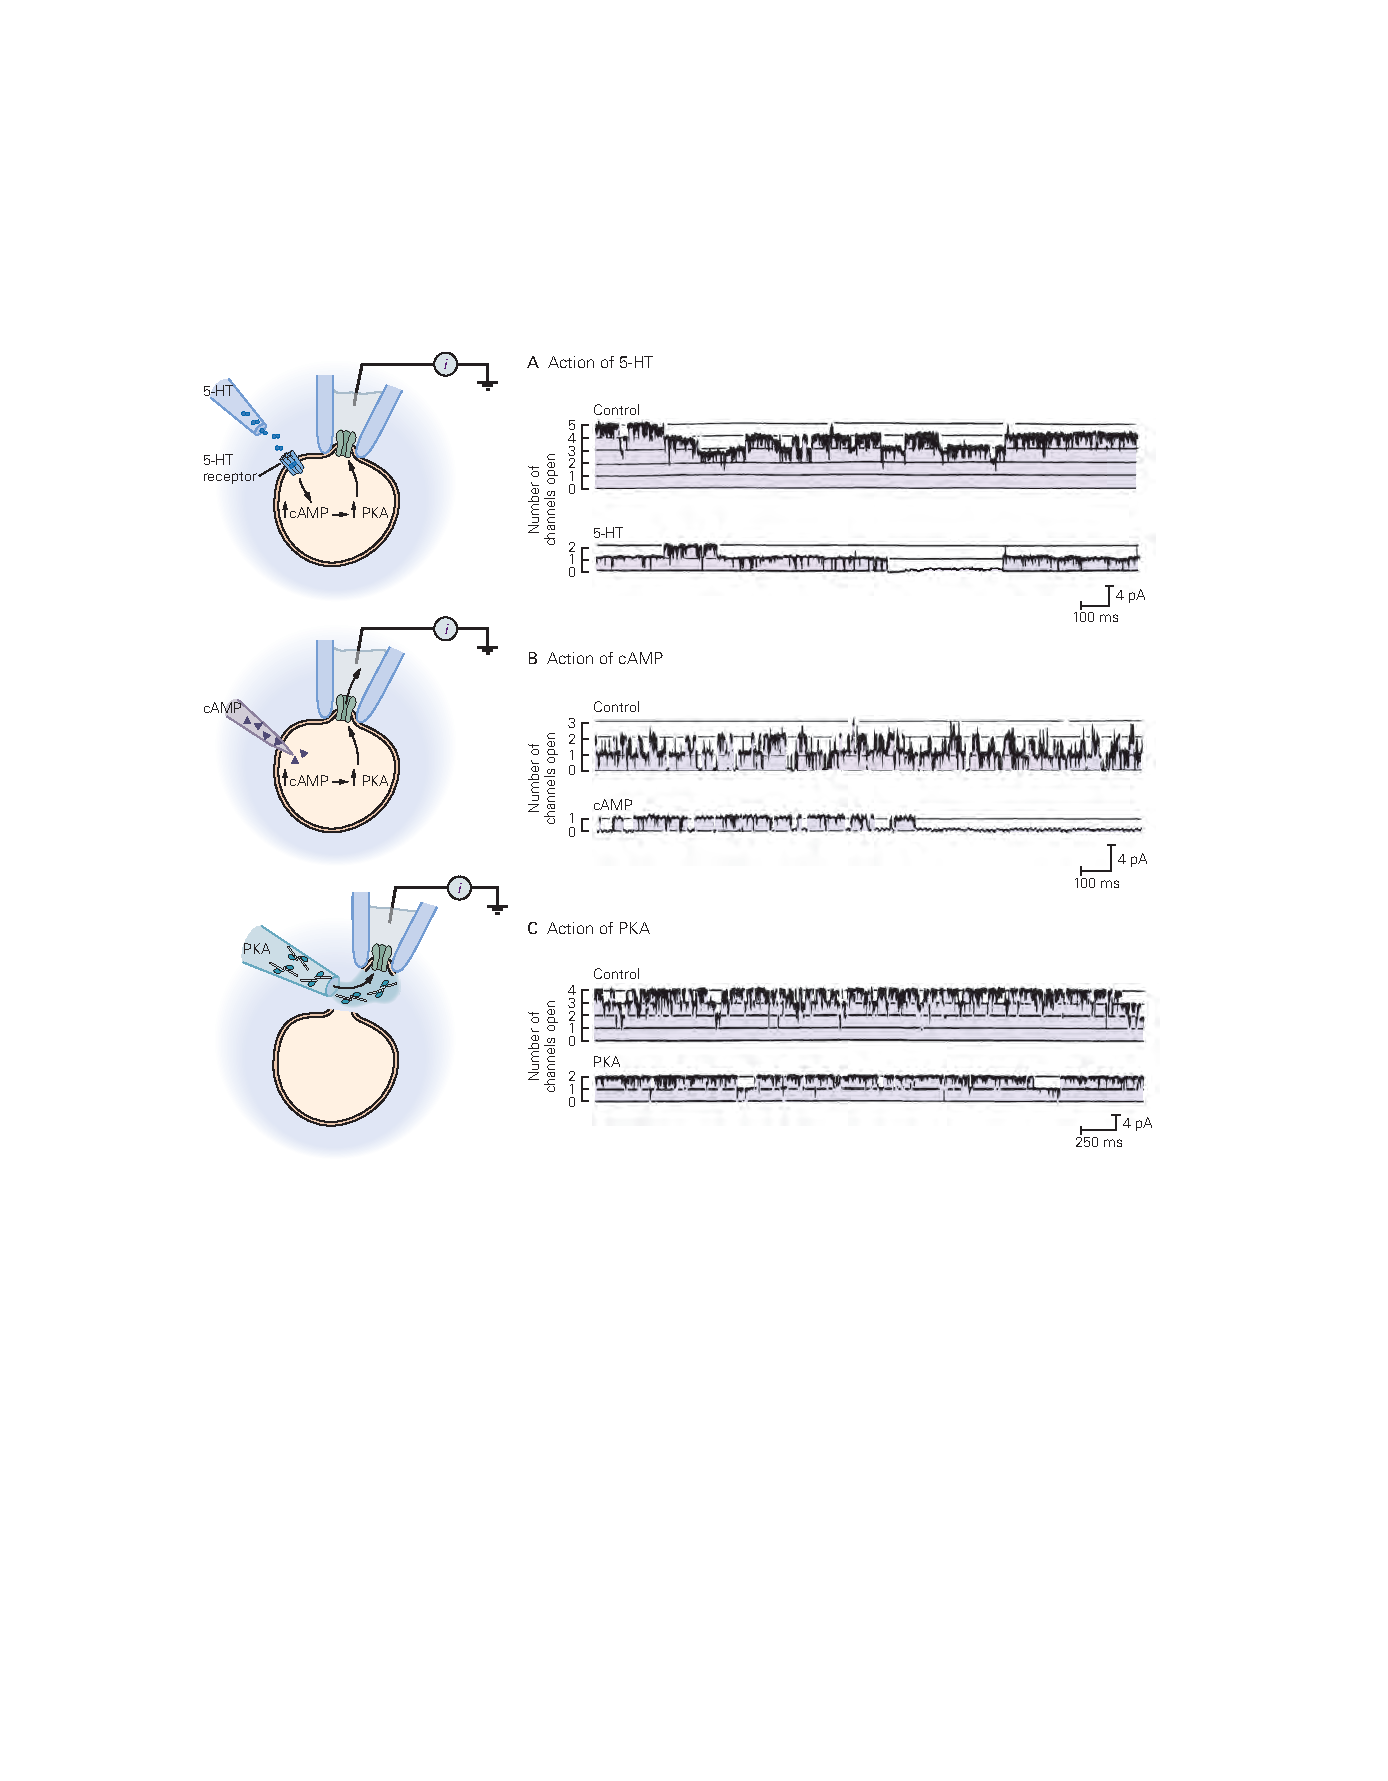
\includegraphics[width=0.85\linewidth]{chap14/fig_14_11}
	\caption{血清素能中间神经元通过可扩散的第二信使\textit{环磷酸腺苷}关闭 \ce{K+} 通道。
		\textit{5-羟基色氨酸}通过关闭血清素敏感或 S 型\ce{K+} 通道,在海兔感觉神经元中产生缓慢的\textit{兴奋性突触后电位}。
		\textit{5-羟基色氨酸}受体与刺激腺苷酸环化酶的 $ G_s $ 偶联。
		\textit{环磷酸腺苷}的增加激活了\textit{环磷酸腺苷}依赖性\textit{蛋白激酶A},后者磷酸化 S 型通道,导致其关闭。
		单通道记录说明了\textit{5-羟基色氨酸}、\textit{环磷酸腺苷}和\textit{蛋白激酶A}在 S 型通道上的作用。
		\textbf{A. }将\textit{5-羟基色氨酸}添加到浴中会关闭在这个细胞贴附膜片中活跃的五个 S 型 \ce{K+} 通道中的三个。
		该实验涉及可扩散信使,因为在浴中应用的\textit{5-羟基色氨酸}无法直接进入移液器下方膜中的 S 型通道。
		每个通道开口都会产生一个向外(正)电流脉冲\cite{siegelbaum1982serotonin}。
		\textbf{B.} 通过微电极将\textit{环磷酸腺苷}注射到感觉神经元中会关闭此贴片中的所有三个活跃的 S 型通道。
		底部轨迹显示在\textit{环磷酸腺苷}存在的情况下最终活动通道的关闭\cite{siegelbaum1982serotonin}。
		\textbf{C.} 将纯化的\textit{蛋白激酶A}催化亚基应用于膜的细胞质表面,关闭了该无细胞贴片中四个活性 S 型 \ce{K+} 通道中的两个。
		将\textit{三磷酸腺苷}添加到沐浴膜内表面的溶液中,为蛋白质磷酸化提供磷酸盐来源\cite{shuster1985cyclic}。}
	\label{fig:14_11}
\end{figure}


因此,单个通道可以由不同的第二信使通路调节,这些通路对神经元兴奋性产生相反的影响。
同样,在哺乳动物神经元的每个亚基(TREK-1 通道)中具有两个成孔结构域的静息\ce{K+}通道受到\textit{蛋白激酶A}和花生四烯酸的双重调节,其方式与海兔中 S 型通道的双重调节非常相似。



\section{第二信使可以赋予突触传递持久的影响}

到目前为止,我们已经描述了突触第二信使如何在持续数秒到数分钟的时间内改变神经元的生物化学。
由于细胞特定基因表达的改变,第二信使还可以产生持续数天至数周的长期变化(图~\ref{fig:14_12})。 
基因表达的这种变化是由于第二信使级联控制转录因子活性的能力,转录因子是控制\textit{信使核糖核酸}合成的调节蛋白。


\begin{figure}[htbp]
	\centering
	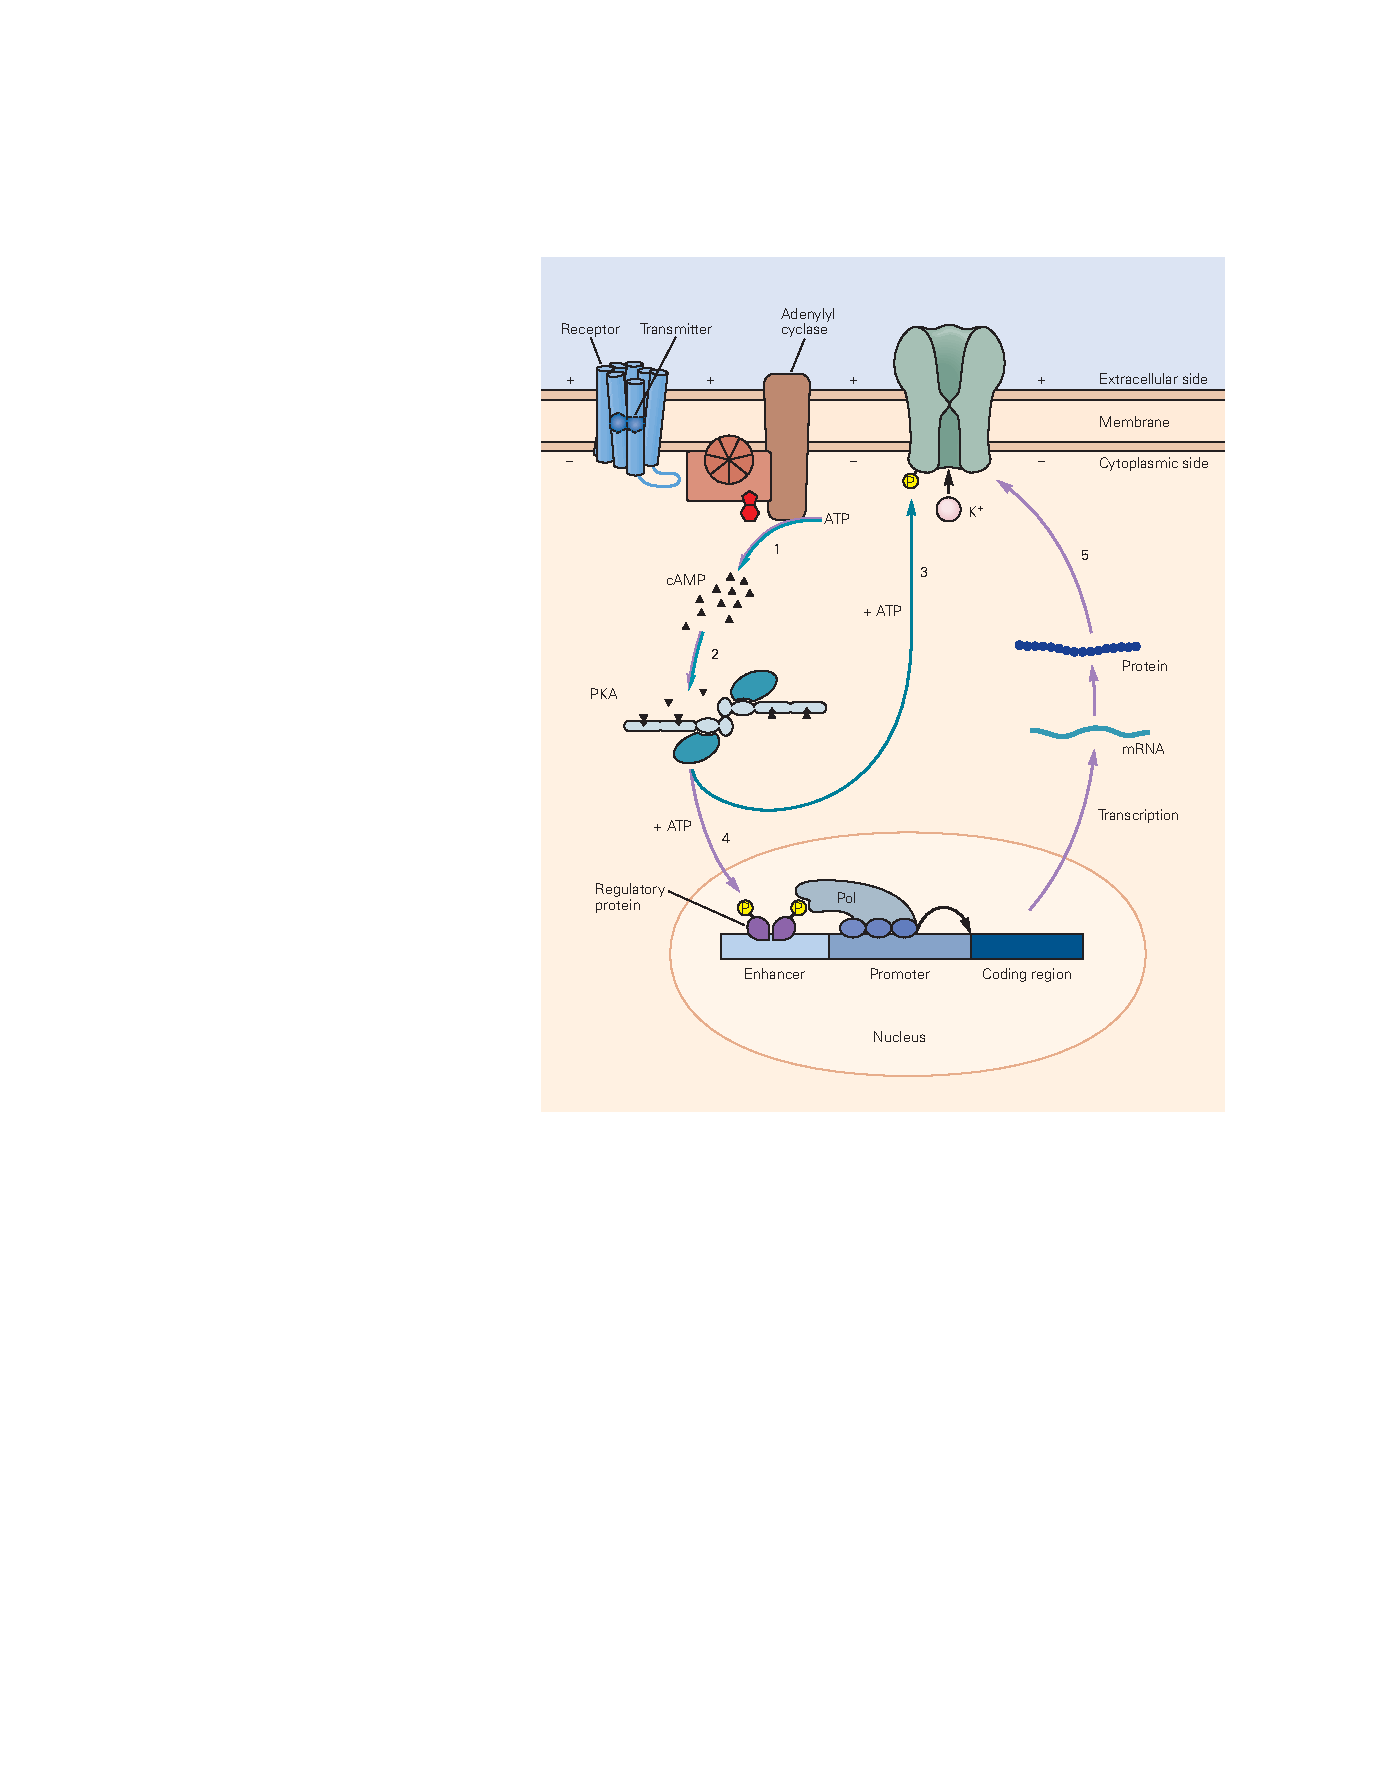
\includegraphics[width=0.7\linewidth]{chap14/fig_14_12}
	\caption{单一的神经递质可以对离子通道产生短期或长期的影响。
		在此示例中,短时间接触发射器会激活\textit{环磷酸腺苷}第二信使系统 (1),进而激活\textit{蛋白激酶A} (2)。
		激酶磷酸化\ce{K+}通道;
		这会导致持续几分钟的突触电位并改变神经元的兴奋性 (3)。
		随着受体的持续激活,激酶转移到细胞核,在那里磷酸化一种或多种开启基因表达的转录因子 (4)。
		作为新蛋白质合成的结果,突触动作被延长——通道的关闭和神经元兴奋性的变化持续数天或更长时间 (5)。
		(Pol,聚合酶。)}
	\label{fig:14_12}
\end{figure}


一些转录因子可以通过磷酸化直接调节。
例如,\textit{环磷酸腺苷}反应元件结合蛋白 (CREB) 在被\textit{蛋白激酶A}、钙/钙调蛋白依赖性蛋白激酶、PKC 或 MAP 激酶磷酸化时被激活。
一旦被激活,CREB 通过结合特定的\textit{脱氧核糖核酸}序列、\textit{环磷酸腺苷}反应元件或 CRE 并募集转录机制的一个组分 CREB 结合蛋白 (CBP) 来增强转录。
CBP 通过募集\textit{核糖核酸}聚合酶 II 和作为组蛋白乙酰化酶发挥作用,向某些组蛋白赖氨酸残基添加乙酰基来激活转录。
乙酰化削弱了组蛋白和\textit{脱氧核糖核酸}之间的结合,从而打开染色质结构并使特定基因能够被转录。
转录和染色质结构的变化对于调节神经元发育以及长期学习和记忆很重要(第~\ref{chap:chap53}~和~\ref{chap:chap54}~章)。



\section{调制器可以通过改变内在兴奋性或突触强度来影响电路功能}

本章的大部分内容致力于理解允许神经调节剂激活的通路改变单个神经元中离子通道、受体和突触活动的细胞机制和信号转导通路。
然而,在完整的大脑中,从大面积大脑区域的扩散投射(第~\ref{chap:chap16}~章)或更多局部目标连接释放的调节性递质可以通过多种重要方式改变大脑回路的动力学。
在本节中,我们研究了一个经过充分研究的回路功能调节控制的例子——口胃神经节神经元对甲壳类动物摄食行为的控制,以说明以下一般特性。


1. 调节投射神经元或神经激素可以协同影响大量神经元的特性,从而改变神经回路或整个动物的状态。
例如,从相对较少数量的神经元释放的调节剂在控制睡眠和觉醒之间的转换中很重要(第~\ref{chap:chap44}~章)。


2. 神经调节剂作用于中间时间尺度,从几毫秒到几小时不等。
快速突触传递和快速动作电位传播非常适合快速计算对行为重要的各种过程。
然而,在较长时间尺度上起作用的调制器可以偏置电路的动态以扩大其动态范围或使其适应动物的行为需求。
例如,许多感觉过程会根据动物的行为状态引起非常不同的反应,而改变突触强度和内在兴奋性的调节剂通常参与此类行为。



\subsection{多种神经调节剂可以汇聚到同一个神经元和离子通道上}

在我们对海兔 S 通道的讨论中,我们已经看到不同的调节剂如何调节相同的离子通道。
这是一个共同的主题,因为 M 型\ce{K+}通道受乙酰胆碱、P 物质和各种其他肽的调节。


一个特别显着的收敛例子是甲壳类动物口胃神经节神经元的调节控制。
在那里,大量结构不同的神经肽汇聚以调节电压依赖性内向电流 (IMI)。
IMI虽然是小电流,但对兴奋性的调节以及平台电位和爆发电位的产生具有重要作用。
许多神经元表达大量不同的受体类型,使这些细胞能够在不同的大脑状态下灵活地响应不同的调节输入。


甲壳类动物口胃神经节 (STG) 包含 26 到 30 个神经元,并产生两种对进食很重要的节律运动模式——胃节律和幽门节律。
一组 STG 神经元产生幽门节律,这对过滤食物很重要,并且在动物的整个生命过程中持续活跃。
另一组神经元产生胃磨节奏,它会在胃内移动三颗用于咀嚼和研磨食物的牙齿。
胃磨节律响应于食物而被激活,因此仅在体内间歇性地活跃。
特定节律在任何时候是否处于活动状态都受到各种神经调节剂的控制,其中一些激活幽门和胃磨机节律,而另一些则抑制它们。
这些调节剂可以在特定的突触接触处释放,或者可以像神经激素一样扩散。
有趣的是,调制器还可以使单个神经元在这两个电路之间切换,从而增加这一小部分神经元可以实现的计算能力。


作为 STG 幽门节律起搏器的基本回路(内核)由单个前爆裂 (AB) 神经元和两个幽门扩张器 (PD) 神经元组成。
两种类型的神经元都与第三种神经元幽门 (PY) 神经元建立抑制性突触连接。
在爆发期间,缓慢去极化的起搏器电位(慢波)会触发 AB 和 PD 神经元中的动作电位爆发。
由于这些神经元被电(间隙连接)突触强烈耦合,它们去极化并同步激发动作电位,导致下游 PY 神经元的瞬态抑制(图~\ref{fig:14_13}A)。


\begin{figure}[htbp]
	\centering
	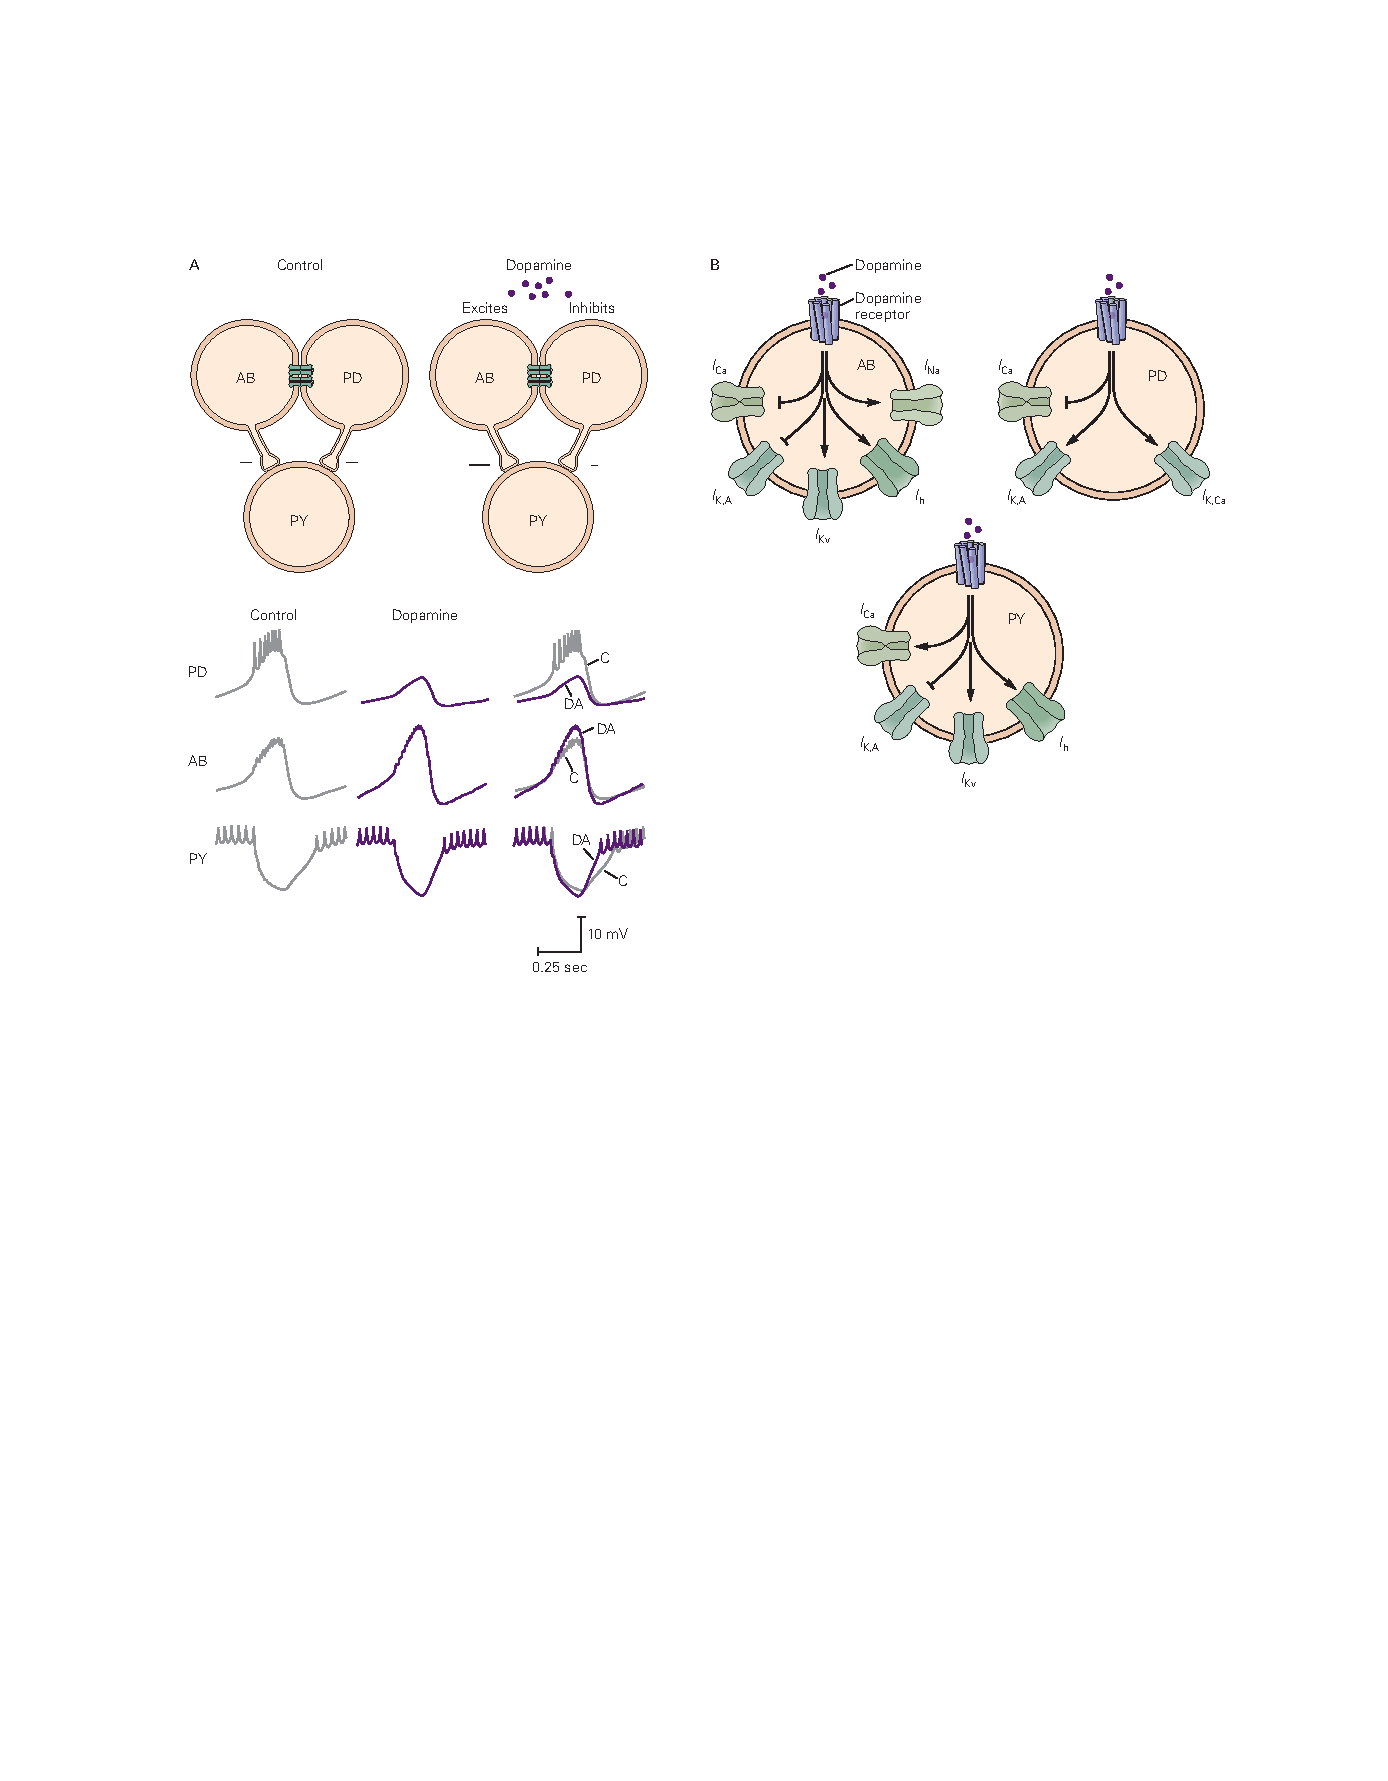
\includegraphics[width=0.95\linewidth]{chap14/fig_14_13}
	\caption{多巴胺对龙虾胃胃神经节幽门节律的调节作用是由多种作用引起的。
		\textbf{A.} 电路图显示了三个幽门电路神经元之间的相互作用。
		前爆裂 (AB) 和幽门扩张器 (PD) 神经元通过间隙连接通道强烈电耦合。
		AB 和 PD 神经元均与幽门 (PY) 神经元形成抑制性突触,从而在该细胞中产生\textit{抑制性突触后电位}。
		细胞内电压记录说明了在没有多巴胺能输入(对照)和有多巴胺的情况下 PD、AB 和 PY 神经元的幽门节律阶段。
		在右侧,叠加了来自对照细胞 (C) 和具有多巴胺能输入 (DA) 的细胞的电压迹线。
		多巴胺增强 AB 神经元中慢波爆发的振幅(在该神经元中,轴突动作电位被神经元的电缆特性高度衰减,并在体细胞中表现为微弱的波纹)但超极化并降低慢波的振幅 PD 神经元中的波。
		这些联合行动导致 PY 神经元中的\textit{抑制性突触后电位}较短,使其能够比 PD 神经元更早地发射\cite{eisen1984mechanism}。
		\textbf{B.} 多巴胺调节 AB、PD 和 PY 神经元中的许多不同的电压依赖性通道。
		这些包括 \ce{Ca^2+} 电流 (ICa)、钙激活 \ce{K+} 电流 (IK,Ca)、失活 \ce{K+} 电流 (IK,A)、延迟整流 \ce{K+} 电流 (IKv)、超极化激活阳离子电流 (Ih) 和 持久的 \ce{Na+} 电流 (INa)。
		带箭头的线表示当前增加,以短线段结尾的线表示当前减少\cite{marder2007understanding,harris2011neuromodulation}。}
	\label{fig:14_13}
\end{figure}


多巴胺在甲壳类动物中作为快速神经递质和神经激素发挥作用,通过作用于许多神经元和突触影响突触强度以及神经元和肌肉兴奋性来影响进食行为。
例如,多巴胺的应用降低了 PD 神经元中的慢波振幅,但增加了 AB 神经元中慢波的振幅。
Ron Harris-Warrick 发现多巴胺调节两个神经元中不同的膜电流组,提供了一个清楚的例子,说明单个调节递质如何在不同的突触后细胞中发挥不同的作用(图~\ref{fig:14_13}B)。


多巴胺还会改变这些神经元活动的相对时间。
尽管 PY 神经元接收来自 AB 和 PD 神经元的抑制性输入,但来自 AB 神经元的抑制性突触作用比来自 PD 神经元的抑制性突触作用更快。
因此,多巴胺通过抑制 PD 神经元和抑制 IPSP 的慢速成分,加速 PY 神经元中联合\textit{抑制性突触后电位}的时间进程(图~\ref{fig:14_13}A),有助于改变 PY 神经元的活动时间 PY 神经元相对于起搏器组。
多巴胺还通过降低瞬态 A 型\ce{K+}电流 (IK,A) 同时增加 HCN 通道 (Ih) 携带的兴奋性慢内向电流 (Ih) 来调节其内在兴奋性,从而增强 PY 神经元的放电(图~\ref{fig:14_13}B)。
因此,调制器对电路的影响源于其对分布式电路元件中许多电压门控通道和突触的选择性作用。



\subsection{为什么有这么多调制器?}

我们现在知道 STG 是 50 种或更多不同神经调节物质的直接目标,包括生物胺、氨基酸、\textit{一氧化氮}和大量神经肽,它们从下行调节投射神经元和感觉神经元释放,并作为激素在大脑中循环 血淋巴。
许多这些调节剂作为共递质从某些被感觉神经元激活的下行纤维的末端释放。
许多神经调节剂都在 STG 神经细胞中以突触方式释放,并且还起到神经激素的作用。


为什么一个只有 26 到 30 个神经元组成的小神经节要受到这么多物质的调节?
起初,人们认为调节神经支配的丰富性对于产生不同的行为相关运动输出很重要。
这仍然是正确的,但现在也很明显,一些调制器可能专门用于特殊情况,例如蜕皮,并且具有相似效果的不同调制器确保即使失去一个调制系统也能保留重要功能。
因此,可以使用不同的调制器来服务于可塑性和稳定性。



\section{亮点}

1. 神经调节剂是与受体结合的物质,其中大部分是代谢型的,以改变神经元的兴奋性、递质释放的可能性或突触后神经元受体的功能状态。


2. 当神经调节剂激活第二信使通路时,调节剂可以影响离释放位点一定距离的离子通道和其他目标的特性。


3. 一些神经调节系统对许多神经元和许多大脑区域具有广泛而显着的作用。


4. 有两个主要的\textit{代谢型受体}家族:
G 蛋白偶联受体和受体酪氨酸激酶。 
许多重要的大脑信号分子,如去甲肾上腺素、\textit{乙酰胆碱}、GABA、谷氨酸、血清素、多巴胺和许多不同的神经肽,激活\textit{代谢型受体};
许多这些相同的物质也会激活离子受体。 


5. 循环 AMP 途径是最了解的第二信使信号级联反应之一。
\textit{代谢型受体}激活会触发一系列生化反应,导致腺苷酸环化酶的激活,后者合成\textit{环磷酸腺苷},进而激活蛋白激酶 A。
该激酶随后磷酸化目标蛋白,改变其功能状态。
\textit{蛋白激酶A}的重要目标包括电压和配体门控离子通道以及对囊泡释放很重要的蛋白质。 


6. 磷脂酶 C 水解磷脂产生 DAG 和\textit{肌醇1,4,5-三磷酸}它们在细胞内 \ce{Ca^2+} 处理中起重要作用。
内源性大麻素由脂质前体合成,可以作为逆行信使跨突触起作用。
另一种广义信号分子是气体一氧化氮,它扩散穿过细胞膜并刺激循环 GMP 合成。


7. 受体酪氨酸激酶也间接门控离子通道以响应结合多种肽激素。 


8. 神经调节剂可以关闭离子通道,从而降低膜电导。
M 型电流是一种缓慢激活的电压门控 \ce{K+} 电流,是动作电位适应的基础。
\textit{乙酰胆碱}和几种神经肽会降低 M 型电流幅度,从而产生缓慢的去极化并降低适应性。
S 型 \ce{K+} 通道有助于某些神经元的静息 \ce{K+} 电导,包括一类介导海兔鳃退缩反射的感觉神经元。
血清素通过\textit{环磷酸腺苷}信号级联关闭通道,使静息膜去极化,增加兴奋性,并增强感觉神经元末梢的递质释放。
长时间接触血清素会改变基因转录,从而导致突触强度发生长期变化。 


9. 调制器可以通过作用于众多电路目标来改变神经元电路的输出。 


10. 鉴于所有大脑神经元和突触都可能被一种或多种物质调节,值得注意的是大脑回路很少会“过度调节”以致于失去功能。
需要更多的研究来理解在允许网络可塑性的调制器面前允许稳健和稳定的网络性能的规则。


11. 除了小神经节或视网膜等少数值得注意的情况外,我们很可能仍然只有部分存在和活跃的神经调节物质总数的目录。


12. 我们对神经调节作用的了解大部分来自体外研究。
关于如何在行为动物中控制神经调节浓度,人们知之甚少。





